% original by Dr Kelly Homan

% hosted project:
% http://code.google.com/p/missouri-science-technology-latex-dissertation-thesis-template/

% email list:
% S&T Thesis/Dissertation LaTeX Template User Group <latextdt-grp@mst.edu>

% google group:
% https://groups.google.com/a/mst.edu/group/latextdt-grp/topics?hl=en

% see http://grad.mst.edu/currentstudents/thesesdissertations/
% for guidelines
\documentclass[times,12pt,titlepage]{mstthesis} % 
\doublespacing
% Dr Parris, Vojta, Story, and Yamilov would prefer single spaced, double sided print
% Binding and printing: 
% Library needs good paper, bound. Department can uses either good or normal paper, also bound. Department will pay for binding of these two copies.
% Dr Yamilov wants two copies on good paper, single spaced and double sided; bound (one for him, one for Hui Cao). Cost of binding is $10 per copy through department. 
% Parents printed copy

% Ben isn't sure what the purpose of the following are
\usepackage{fancyhdr}
\pagestyle{fancy}
\lhead{}\chead{}\rhead{\thepage}
\lfoot{}\cfoot{}\rfoot{}
\renewcommand{\headrulewidth}{0pt}
\renewcommand{\footrulewidth}{0pt}

% Ben's additions
\usepackage{comment} % multi-line comments
\usepackage{graphicx} % necessary for inclusion of .eps for figures
\usepackage{algpseudocode}
\usepackage{amsmath}

%Find the pictures
\graphicspath{ {./images/} {./gnuplots/} }

% the following is for published chapters to note where they were published
\renewcommand{\thefootnote}{\fnsymbol{footnote}}
% http://help-csli.stanford.edu/tex/latex-footnotes.shtml

% Use the first command below if you want captions over 1 line indented. A side
% effect of this is to remove the use of bold for captions. To restore bold,
% also include the second line below.
\usepackage[hang]{caption}  
% change the caption delimiter in caption2.sty from a colon to a period:
%\renewcommand\captionlabeldelim{.}
%\usepackage{hangcaption}

% % \usepackage{algorithmic}
% % \usepackage{algorithm}
% % \usepackage{url}
% % \usepackage{lscape}
% % \usepackage{subfigure}
% % \usepackage{flafter} % http://stackoverflow.com/questions/547508/in-latex-is-there-a-way-to-put-a-float-automatically-after-where-it-is-first-re
% % 
% % 
% % %%\ExecuteOptions{textures}

%\usepackage{titlesec}% http://ctan.org/pkg/titlesec
%\usepackage{lipsum}% http://ctan.org/tex-archive/macros/latex/contrib/lipsum   http://ctan.org/pkg/lipsum

%\usepackage{tocloft} % http://ctan.org/pkg/tocloft

% http://en.wikibooks.org/wiki/LaTeX/Page_Layout#Widows_and_orphans
\widowpenalty=10000 % prevents the first line of a paragraph from being alone at the bottom of a page. It will either cause that line to move to the next page, or cause one line from the next page to join the lone line. 
\clubpenalty=10000  % prevent the last line of a paragraph to be alone at the top of a page. At best it will force there to be two lines. 
% MS&T Office of Grad Studies says ``Need to have at least 2 lines at the top and at the bottom of every page. No lone headers at bottom of page.
% see https://groups.google.com/d/msg/comp.text.tex/uN7tvjubk8o/kcUvevut0hEJ

% brokenpenalty is meant to eliminate hyphenation of words at the end of a page. However, it may introduce non-uniform pages
% https://groups.google.com/d/msg/comp.text.tex/pBSOMuQzOH0/innVfjc3ZG4J
\brokenpenalty=10000 % having this causes page numbers to be incorrect in ToC. Not having it causes word breaks at end of page
% better solution, as per Gerry Howser:
%\raggedbottom
% However, it doesn't fix hyphenation at end of page

% http://en.wikibooks.org/wiki/LaTeX/Formatting#Hyphenation
%\hyphenation{local-ization diff-usion}

%\usepackage{enumerate}

% for T/E paper
%\usepackage{graphicx}
\usepackage{epsfig}
\usepackage{color}
\usepackage{verbatim} % multi-line comments

% for D(z) PRB
% % %\usepackage[fleqn]{amsmath}
% % %\usepackage{amsthm}
%\usepackage{amsmath} % adding this doesn't fix the symbol problem, as the package is required by mstthesis.cls
%\usepackage{mathtools} % this 
\usepackage{amssymb} % \gtrsim

\usepackage{makeidx} % Index
\makeindex
%\usepackage{glossary}
\usepackage[xindy,toc]{glossaries} % http://en.wikibooks.org/wiki/LaTeX/Glossary
\makeglossary  % http://texblog.wordpress.com/2007/11/01/glossary-in-latex/

% Note: hyperref must be the last package
\usepackage[breaklinks=true, % allow links to break over lines by making links over multiple lines into PDF links to the same target 
% hyperindex, % Makes the page numbers of index entries into hyperlinks. 
% %backref, 
%pdftex,
%bookmarks=true % bookmark hierarchy is incorrect   http://www.latex-community.org/forum/viewtopic.php?f=47&t=7762
%bookmarksnumbered=true
% %pagebackref, % Adds backlink text to the end of each item in the bibliography, as a list of page numbers. 
linktocpage, % make page number, not text, be link on TOC, LOF and LOT 
% colorlinks=false, 
pdftitle={Comprehensive}, 
pdfauthor={Stephen Jackson}, 
pdfsubject={PhD Comprehensive}, 
pdfkeywords={exam jackson distributed systems smart grid leader election group management}
]{hyperref}

%ps% ... uncomment after editing toc, lof, lot ...
%ps%\nofiles
\usepackage{subfigure}             % allows for use of "sub figure" 1a, 1b, etc

\begin{document}

%ps% ... specify: ms | phd ...
\begin{ThesisTitlePage}{phd}

\author{\MakeUppercase{Stephen Jackson}}

\thesistitle{Applications for Group Management To Manage CPS Stability}

\department{Computer Science}

\degree{Doctor of Philosophy}

%ps% ... thesis committee ...

\ThesisAdviser{Dr. Bruce McMillin}

%ps% If you have a co-advisor, enter the name in the
%ps% curly braces below and uncomment.
%ps% Otherwise, leave commented out.
%ps%\cothadviser{} % If you have 2 thesis advisers

\memberone{Dr. Alireza Hurson}
\membertwo{Dr. Wei Jiang}
\memberthree{Dr. Sriram Chellappan}
\memberfour{Dr. Sahra Sedighsarvestani}

%ps% ... Graduation date.  NOT your submission date! ...
\graddate{2014}

\end{ThesisTitlePage}

%ps% ... copyright page - true|false ...
% from 
% http://creativecommons.org/choose/

%This work is licensed under the Creative Commons Attribution-NonCommercial-ShareAlike 3.0 Unported License. To view a copy of this license, visit 
%\\\mbox{\href{http://creativecommons.org/licenses/by-nc-sa/3.0/}{http://creativecommons.org/licenses/by-nc-sa/3.0/}} 
%or send a letter to Creative Commons, 444~Castro Street, Suite~900, Mountain View, California, 94041, USA.

%\ \\
%Published journal articles retain their original copyrights.

% http://www.tandf.co.uk/journals/contact.asp
% Customer Services for Taylor & Francis Group Journals
% T&F Customer Services
% 325 Chestnut Street
% Suite 800
% Philadelphia, PA 19106, USA
% 
% http://journalauthors.tandf.co.uk/preparation/copyright.asp
% 
% "the right to include an article in a thesis or dissertation that is
% not to be published commercially, provided that acknowledgement to
% prior publication in the relevant Taylor & Francis journal is made
% explicit;"
% 
% 
% ****************************
% APS Headquarters
% One Physics Ellipse
% College Park, MD 20740-3844
% (301) 209-3200
% 8am-6pm M-F
% 
% http://publish.aps.org/copyrightFAQ.html#thesis
% 
% "As the author of an APS-published article, may I include my article
% or a portion of my article in my thesis or dissertation?"
% 
% "Yes, the author has the right to use the article or a portion of the
% article in a thesis or dissertation without requesting permission from
% APS, provided the bibliographic citation and the APS copyright credit
% line are given on the appropriate pages."
% 
% ****************************
% Elsevier: 1 888 834 7287
% 
% http://www.elsevier.com/wps/find/authorsview.authors/rights
% 
% "the right to include the journal article, in full or in part, in a
% thesis or dissertation;"

\copyrightyear{2013}
\ThesisCopyrightPage{false}

%ps% ... front matter - publication option - ms|phd...

%\begin{ThesisPublicationOption}{phd}
%This dissertation has been prepared in the form of six papers.

%\renewcommand{\theenumi}{Paper \arabic{enumi}}
%\begin{enumerate}%[Paper 1]

%  http://tex.stackexchange.com/questions/38139/how-can-i-calculate-the-difference-of-2-counters-pageref
% \newcounter{tempor}
% \setcounter{tempor}{\pageref{paper:1_start}}
% \addtocounter{tempor}{1}
%\item Pages~\arabic{temp}--\pageref{paper:1_end} have been published as
%\item Pages~\pageref{paper:1_start}--\pageref{paper:1_end} have been published as 
%  \textit{\href{http://link.aps.org/doi/10.1103/PhysRevB.82.104204}{Relation between transmission and energy stored in random media with gain}}, Physical Review B \textbf{82} 104204 (2010) with Jonathan Andreasen, Hui Cao, and Alexey Yamilov.
%\item Pages~\pageref{paper:2_start}--\pageref{paper:2_end} have been published as 
%  \textit{\href{http://dx.doi.org/10.1080/09500340.2010.519443}{Classification of regimes of wave transport in non-conservative random media}}, Journal of Modern Optics (2010) with Alexey Yamilov.
%\end{enumerate}
%\renewcommand{\theenumi}{\arabic{enumi}}

%An earlier letter, 
%\textit{\href{http://dx.doi.org/10.1016/j.physb.2010.01.025}{Criterion for light localization in random amplifying media}}, 
%has been published in Physica B \textbf{405}, 3012--3015 (2010) with Hui Cao and Alexey Yamilov. This is reported in Paper 1.

%\end{ThesisPublicationOption}
%ps% ... front matter - thesis abstract ...
\begin{ThesisAbstract}
\begin{abstract}
\begin{abstract}
Cyber-physical systems (CPS) are an attractive option for future development of
critical infrastructure systems. By supplementing the traditional physical
network with cyber control, the performance and reliability of the system
can be increased. In some of these networks, distributing the cyber control
offers increased redundancy and availability during fault conditions. However,
there are very few works which study the effects of cyber faults on a 
distributed cyber-physical system. These are of a particular interest in the smart grid
environment where outages and failures are very costly. By examining the
behavior of a distributed system under fault scenarios, the overall robustness
of the system can be improved by planning characteristics and responses to
faults that allow the system to continue operating in difficult circumstances.

This work examines the consequences of network unreliability on a core part of the
 Distributed Grid Intelligence (DGI) for the FREEDM (Future Renewable Electric 
Energy Delivery and Management) Project. By applying different rates of packet
loss in specific configurations to the communication stack of the software and
observe the behavior of a critical component (Group Management) under those
conditions. These components identify the amount of time spent in a group,
working, as a function of the network reliability. Given this one can parameterize
the amount of messages that are lost and thus the number of failed physical actuations.
Knowing this and the physical characteristics of the system, one can tune the amount
of time between reconfiguration in order to prevent the number of failed physical
changes from causing the system to become unstable. Using this, we can develop
methods and guarantees to protect the operation of a CPS.
\end{abstract}

\end{abstract}
\end{ThesisAbstract}

%ps% ... front matter - acknowledgements ...
\begin{ThesisAcknowledgment}
The author acknowledges the support of the Future Renewable
Electric Energy Delivery and Management Center,
a National Science Foundation supported Engineering Research
Center under grant NSF EEC-081212, and the United States Department of Education GAANN program.

\end{ThesisAcknowledgment}

%ps% ... toc, lof, and lot (list of symbols in respective papers) ...
\begin{ThesisFrontMatter}
\tableofcontents
\listoffigures
\listoftables
\end{ThesisFrontMatter}

\newcommand{\boldnabla}{\mbox{\boldmath$\nabla$}}
\newcommand{\boldrho}{\mbox{\boldmath$\rho$}}

%ps% ... chapter 1 - ptointroduction ...
\begin{ThesisBody}
%Here is dissertation body
% Introduce the contents of the paper and what will be presented
\chapter{Introduction}

The design of stochastic models of distributed systems has a long history as a challenging area of interest.
Models of distributed systems have to deal with a number of factors.
These factors include the various types of failure the system could experience, a lack of tightly synchronized execution, and a large complex state space when there are a high number of agents\cite{DISTRIBUTED}\cite{distributed-challenges}. 
However, the concept of distributed systems plays a central role in many of the future visions for how critical infrastructure will operate.
These critical infrastructures are physical networks whose operation are so vital that if those networks failed to operate correctly it would be highly detrimental to the population that rely on those systems.
\ac{CPS} are the integration of computational systems with physical networks.
Computational systems already play a critical role in most critical infrastructures, and as demands for security features, such as accessibility, increase distributed systems are becoming an increasingly favorable choice for the computational needs for these systems\cite{SMARTGRIDBENEFITS}.

The \ac{FREEDM} center\cite{FREEDM}, an NSF funded ERC envisions a future power-grid where widely distributed renewable power generation and storage is closely coupled with a distributed system that facilitates the dispatch of power across those areas.
Other systems like \ac{VANET}\cite{CARS1}\cite{CARS2}\cite{vanet-congestion} and air traffic control systems\cite{AIRTRAFFIC1}\cite{AIRTRAFFIC2} also propose similar control systems where many computers must cooperate to ensure both smooth operation and the safety of the people using those systems.
As a consequence, ensuring that the computer systems that control those infrastructures behave correctly during fault conditions is critical, especially when those computer systems rely on their interaction with other computers to operate.

A robust \ac{CPS} should be able to survive and adapt to communication network outages in both the physical and cyber domains.
When one of these outages occurs, the physical or cyber components must take corrective action to allow the rest of the system to continue operating normally.
Additionally, processes may need to react to the state change of some other process.
Managing and detecting when other processes have failed is commonly handled by a leader election algorithm and failure detector.

In a smart-grid system, misbehavior during fault conditions could lead to critical failures such as a blackout or voltage collapse. In a \ac{VANET} or air traffic control system, vehicles could collide, injuring passengers or destroying property. Additionally, since these systems are a part of critical infrastructure, protecting them from malicious entities is an important consideration.

This work was motivated by observations on the effects of lost messages on the group management module of the \ac{DGI} used by the \ac{FREEDM} smart-grid project.
These original observations confirmed the need to explore more well defined models for the behaviors of \ac{CPS} in order for them to better serve the people that use them.

We present a framework for reasoning about inferable state in the context of a distributed system. To do this, we exploit existing work in the field of information flow security. Information flow security has been used to reason about how attacks like STUXNET can manipulate operators beliefs while disrupting a system\cite{STUXNET}. In particular, these approaches reason about how the operator in a STUXNET attack has no avenue to verify the reports from a compromised computing device. Using existing modal logic frameworks and using information flow security models\cite{Howser2012}\cite{STUXNET}\cite{Howser2013}, one can formally reason about where information that is not normally known to a domain can be inferred.

We will show in this work that in a system with the correct information flows, an agent in a distributed system can infer the state of other agents in the system. With this information, that agent can then construct a reasonable model of the system to determine if the current behavior could lead to an undesirable situation with either the cyber or physical network.

Using this framework we present a leader election algorithm that can be modeled with a Markov chain for a known omission fault\cite{OMISSIONFAILURES} rate.
The presented algorithm maintains the Markov property for the observations of the leader despite omission faults.
This approach to considering how a distributed system interacts during a fault condition allows for the creation of new techniques for managing a fault scenario in cyber-physical systems.
In the context of \ac{FREEDM}, these models produce expectations of how much time the DGI will be able to spend coordinating and doing useful work.
Using these measures, the behavior of the control system for the physical devices can be adjusted to prevent faults, like blackouts and voltage collapse, in the physical network.

We also propose using existing schemes to detect communication network congestion and inform processes in a \ac{CPS} of impending congestion.
Processes act on this information to change their behavior in anticipation of message delays or loss.
This behavior allows them to harden themselves against the congestion, and allows them to continue operating as normally as possible during the congestion.
This technique involves changing the behavior of both the leader election\cite{INVITATIONELECTION} and physical device management algorithm during congestion.

To accomplish this, we extend existing networking concepts of \ac{RED}, \ac{ECN}\cite{RFCECN}, and ICMP source quench\cite{RFCSOURCEQUENCH}.
When a network device detects congestion, it notifies processes that the network is experiencing congestion and they should react appropriately.
We demonstrate an implementation of the \ac{FREEDM} \ac{DGI} in a \ac{NS3} simulation environment\cite{NS3} with our congestion detection feature.
The \ac{DGI} operates normally until the simulation introduces a traffic flow that congests the network devices in the simulation.
After congestion has been identified by the \ac{RED} queuing algorithm, the \ac{DGI} are informed. %via UDP multicast.
When the congestion notifications are introduced, the \ac{DGI} maintains configurations which they would normally be unable to maintain during congestion.
Additionally, we show a greater amount of work can be done without the work causing unstable power settings to be applied.



\chapter{Related Work}

\section{Failure Classification}

Processes can fail in a variety of ways. In this work we focus on how cyber processes can fail. There are a variety of faults that have been classified. In this work,
we focus on two different modes of failure:

\subsection{Crash or Fail-Stop Failure}

A crash failure or its more generalized form, a fail-stop failure, describes a failure in which a process stops executing. In general, this is considered to be an
irreversible failure, since a process typically does not resume from a crashed state. There are categorizations of crash failures, called napping failure
where a process will appear to have crashed for a finite amount of time before resuming normal operation. Crash failures are impossible to detect with absolute
certainty in an asynchronus system. Processes can be suspected by other processes through the use of challenge/response messages or heartbeat messages that allow
a process to prove that it has not crashed yet. A system that can handle a crash failure is implied to be able to handle a fail-stop failure.\cite{DISTRIBUTED}

The fail-stop failure has three properties \cite{DISTRIBUTED}:

\begin{enumerate}
\item When a failure occurs the program execution is stopped.
\item A process can detect when another fail-stop process has failed.
\item Volatile storage is lost when the fail-stop process is stopped.
\end{enumerate}

\subsection{Omission Failure}

An omission failure occurs when a message is never recieved by the reciever. Omission failures can occur when the communication medium is unavalable,
or when the latency of message exceeds a timeout for it's expected delivery. Protocols like TCP do not tolerate omission failures: a packet is resent until
it is acknowledged by the reciever. If the acknowledgement never comes, the connection is closed. As a contrast, UDP assumes that any datagram could be lost
and it is the responsibility of the programmer to handle missing datagrams appropriately. An omission failure can have the same observable affects as a napping
failure in some situations. \cite{DISTRIBUTED}

\section{Virtual Synchrony}
Virtual synchrony (and its original implementation, Isis\cite{ISISTOOLKIT}) is an execution model for distributed systems. Virtual synchrony is based on the idea of synchronous execution where each process acts based on a globally shared clock. Synchronous systems are the easiest to program for, but true synchrony is not feasible in most circumstances. Instead, the virtual synchrony execution model was developed. 

Virtual synchrony is a model of communication and execution that allows the system designer to emulate synchronous execution. Although the processes do not execute tasks simultaneously, the execution history of each process cannot be differentiated from a trace where tasks are executed simultaneously. 

Consider a distributed system where events can be causally related based on their execution on the local processors and communication between processes, as defined in \cite[p~.101]{ISISTOOLKIT}. 

\begin{enumerate}
	\item Let $e \rightarrow e'$ be a casual relationship between events $e$ and $e'$
    \item If $e$ and $e'$ are events local to a process $P_{i}$ and $e$ occurs before $e'$, then $e \rightarrow e'$
    \item If $e = send(m)$ and $e'=deliver(m)$ for the same message $m$, then $e \rightarrow e'$
\end{enumerate}

This defines a dependence and causality relation between events in the system. If two events cannot be causally related (that is $e \not\rightarrow e'$ and $e' \not\rightarrow e$ then the events are considered concurrent. From this, one can define an execution history $H$. A pair of histories $H$ and $H'$ are equivalent if, the history of a process $p$, $H|_{p}$, cannot be differentiated from another history, $H'|_{p}$, based on the casual relationships between the events in the history. \cite[p~.103]{ISISTOOLKIT} Additionally, a history is considered complete if all sent messages are delivered and there are no casual holes. A casual hole is a circumstance where an event $e$ is casually related to $e'$ by $e' \rightarrow e$ and $e$ appears in a history, but $e'$ does not. A virtually synchronous system is one where each history in the system is indistinguishable from all histories produced by a synchronous system. \cite[p~.104]{ISISTOOLKIT}

\subsection{Process Groups}
Virtual synchrony models also support process groups. Although each implementation of a virtually synchronous system applies a different structure to the way processes are grouped, implementations share common features.
A process group in a virtual synchronous system is commonly referred to as a view. A view is a collection of processes that are virtually synchronous with each other. A view refers to a specific group: the set of processes in that view, and a leader if there is one. A group is a general descriptor for a collection of processes. Process groups in virtually synchronous systems place obligations on the delivery of messages to members of a view. A history $H$ of a view is legal if \cite[p~.103]{ISISTOOLKIT}:
\begin{enumerate}
    \item Given a function $time(e)$ that returns a global time of when the event occurred $e$, then $e \rightarrow e' \Rightarrow time(e) < time(e').$
    \item $time(e) \neq time(e') \forall e, e' \in H|_{p}$ (where $e \neq e'$) for each process.
    \item A change in view (group membership) occurs at the same logical time for all processes in the view.
    \item All multicast message deliveries occur in the current view of a group. That is, if a message is sent in a view, it is delivered in that view, for every process in that view.
\end{enumerate}

A process group interacting via message passing creates a legal history for the virtually synchronous system. However, processes can fail.  Virtual synchrony systems have several properties to handle fail-stop failures\cite[p~.102]{ISISTOOLKIT}:

\begin{itemize}
    \item The system employs a membership service. This service monitors for failures and reports them to the other processes in the view.
    \item When a process is identified as failing it is removed from the groups that it belongs to and the remaining processes determine a new view.
    \item After a process has been identified as failing, no message will be received from it.
\end{itemize}

Virtual synchrony's failure model uses the fail-stop failure model. Virtual synchrony does not guarantee how messages will be delivered while transitioning between views. Virtual synchrony only guarantees that view changes are totally ordered with respect to the regular messages sent in the view. A message first sent in an old view may be delivered in a new view. If partitions were allowed to join, the ordering of messages still outstanding from the original views is ambiguous.

Regular messages in virtual synchrony, those which do not announce view changes, can be casually ordered or totally ordered. Additionally, virtual synchrony supports two classes of multicast delivery guarantees: uniform and non-uniform. The uniform property obligates that if a multicast message is delivered to a process in a view, it is delivered to all processes that view. Non-uniform multicast is a multicast that does not guarantee the uniform delivery property.

\section{Extended Virtual Synchrony}
One of the major shortcomings of the original virtual synchrony model lays in how it handles network partitions. In virtual synchrony, when the network is partitioned, only processes in the primary partition were allowed to continue. Processes that were not in the primary partition could not rejoin the primary partition without being restarted: the process joining the view must be a new process so that there are no message delivery obligations for that process in the view. \cite{EXTENDEDVIRTUALSYNCHRONY} presented an improved version of virtual synchrony, dubbed extended virtual synchrony. Extended virtual synchrony is compatible with the original virtual synchrony, and can implement all the functionality and limitations of the original design. Because it supports virtual synchrony, extended virtual synchrony has become the basis for a number of related frameworks that have been designed since Isis including Horus, Totem, Transis, and Spread.

Extended virtual synchrony places obligations on the message delivery service, described informally below \cite{EXTENDEDVIRTUALSYNCHRONY}:
\begin{enumerate}
	\item As defined in Virtual Synchrony, events can be causally related.
		Furthermore, if a message is delivered, the delivery is casually
		related to the send event for that message. 
	\item If a message $m$ is sent in some view $c$ by some process $p$ then $p$
		cannot send $m$ in some other view $c'$
	\item A view is ``installed'' when process recognizes a change in group membership.
	\item If not all processes install a view or a process leaves a view, a new
		view is created. Furthermore, views are unique and events occur after a
		view's creation and before its destruction. Messages which are delivered
		before a view's destruction must be delivered by all processes in that
		view (unless a process fails). Similarly, a message delivery which occurs
		after the creation of a view must occur after the view is installed by
		every process in the view.
	\item Every sent message is delivered by the process that sends it (unless it
		fails) even if the message is only delivered to that process.
	\item If two processes are in sequential views, they deliver the same set of
		messages in the second view.
	\item If the send events of two messages are casually related, if the
		second of those messages is delivered, the first message is also delivered.
	\item Messages delivered in total order must delivered at the same logical time.
		Additionally, this total order must be consistent with the partial, casual
		order. When a view changes, a process is not obligated to deliver messages
		for processes that are not in the same view.
	\item If one process in a view delivers a message, all processes in that view
		deliver the message, unless that process fails. If an event which delivers
		a message in some view occurs, then the messages that installed that view
		were also delivered.
\end{enumerate}

It also provides additional restrictions on the sending of messages between two different views (Item 2) and an obligation on the delivery of messages (Item 4). The concept of a primary view still exists within the extended virtual synchrony model and is still described by the notion of being the largest view. Since views can now partition and rejoin the primary partition the rules presented above also allow the history of the views with respect to the regular messages in the primary partition to be totally ordered. Additionally, two consecutive primary views have at least one process that was a member of each view.

To join views, processes are first informed of a failure (or joinable partition) by a membership service. Processes maintain an obligation set of messages they have acknowledged but not yet delivered. After being informed of the need to change views, the processes begin buffering received messages and transition into a transitional view. In the transitional view messages are sent and delivered by the processes to fulfill the causality and ordering requirements listed above. Once all messages have be transmitted, received and delivered as needed and the process' obligation set is empty, the view transitions from a transitional view to a regular view and execution continues as normal.

\subsection{Comparison To DGI}

The DGI places similar but distinct requirements on execution of processes in its system. The DGI enforces synchronization between processes that obligates each active process to enter each module's phase simultaneously. This is fulfilled by using a clock synchronization algorithm. The virtual synchrony model, at its most basic, does not require a clock to enforce its ordering.

However, this simplifies the DGI fulfilling its real time requirements.  Processes must be able to react to changes in the power system within a maximum amount of time. These interactions do not require interaction between all processes within the group. Additionally, this allows for private transactions to occur between DGI processes. 

The DGI has also been implemented using message delivery schemes that are unicast instead of multicast, since this is the easiest to achieve in practice. A majority of systems implementing virtual synchrony use a model where local area communication is emphasized, with additional structures in place to transfer information across a WAN to other process groups.

Groups in DGI are not obligated to deliver any subset of the messages to any process in the system. Some of the employed algorithms in DGI need all of the messages to be delivered in a timely manner, but they do not require the same message to be delivered to every process in the current design of the system.

\section{Isis (1989) and Horus (1996)}

A product of Dr. Kenneth Birman and his group at Cornell, Isis \cite{ISISTOOLKIT} and Horus \cite{HORUSTOOLKIT} are two distributed frameworks which are comparable to the DGI. Although these projects are no longer actively developed, Isis is the foundation which all other virtual synchrony frameworks are based.

Isis was originally developed to create a reliable distributed framework for creating other applications. As Isis was one of the first of its kind, the burden of maintaining a robust framework that met the development needs of its users eventually led Birman's group to create a newer, updated framework called Horus, which implemented the improved extended virtual synchrony model. However, Isis and Horus largely implement the same concepts.

Both Horus and Isis are described as a group communications system. They provide a messaging architecture which clients use to deliver messages between processes. The frameworks provide a reliable distributed multicast, and a failure detection scheme. Horus offers a modular design with a variety of extensions which can change message characteristics and performance as needed by the project.

\subsection{Group Model}
In Horus and Isis, a group is a collection of processes that can communicate with one another to do work. Multicasts are directed to the view, and are guaranteed to be received by all members or no members.
Over time, due to failure, the view will change. Since views are distributed concurrently and asynchronously, each process can have a different view. Horus is designed to have a modular communication structure composed of layers, which allows the communication channel to have different properties that will affect which messages will be delivered in the event of a view change. Horus' layers allow developers to go as far to not use the complete virtual synchrony model, if the programmer desires. For example, Horus' modules can implement total order using a token passing layer, or casual ordering using vector clocks.

Isis has limited support for partitioning. In the event that a partition forms, dividing the large group into subgroups, only the primary group is allowed to continue operating. The primary group is selected by choosing the largest partition. Horus, on the other hand implements the extended virtual synchrony model and does not have that limitation.

\section{Transis (1992)}

Transis \cite{TRANSISTOOLKIT} was developed as a more pragmatic approach to the creation of a distributed framework. Transis is developed with the key consideration that, while multicast is the most efficient for distributing information in a view or group of processors (as point to point quickly gives rise to N$^{2}$ message complexity, where $N$ is the number of processes. ) it can be impractical, especially over a wide area network to rely on broadcast to deliver messages. Transis, then considers two components for the network: a local area component and a wide area component.

The local area component, Lansis, is responsible for the exchange of messages across a LAN. Transis uses gateways, called Xporters, to deliver messages between the local views. Transis uses a combination of acknowledgements, which are piggybacked on regular messages to identify lost messages. If a process observes a message being acknowledged that it does not receive then it sends a negative acknowledgement broadcast informing the other members of the view it did not receive that message. In Lansis, the acknowledgement signals that a process is ready to deliver a message. Lansis assumes that all messages can be casually related in a global, directed, acyclic graph and there are a number of schemes that deliver messages based on adherence to that graph.

 

\section{Totem (1996)}

Totem\cite{TOTEMTOOLKIT} is designed to use local area networks, connected by gateways. The local area networks use a token passing ring and multicast the messages, much like Isis and Horus. The gateways join these rings into a multi-ring topology. Messages are first delivered on the ring which they are sent, then forwarded by the gateway which connects the local ring to the wide area ring for delivery to the other rings. The message protocol gives the message total ordering using a token passing protocol. Topology changes are handled in the local ring, then forwarded through the gateway where the system determines if the local change necessitates a change in the wide area ring. Failure detection is also implemented to detect failed gateways.
                                             
\section{Spread}

Spread\cite{SPREADTOOLKIT} is a modern distributed framework. It is designed as a series of daemons which communicate over a wide area network. Processes on the same LAN as the daemons connect to the daemon directly. This is analogous to the gateways in the other distributed toolkits, however, the daemon is a special, dedicated message passing process, rather than a participating process with a special role.

Using a dedicated daemon allows a Spread view to reconfigure less frequently when a process stops responding (which normally correlates to a view change) since the daemons can insert a message informing other processes that a process has left while still maintaining the message ordering without disruption. Major reconfigurations only need to occur when a daemon is suspected of failing.

Spread implements an extended virtual synchrony model. However, message ordering is performed at the daemon level, rather than at the group level. Total ordering is done using a token passing scheme among the daemons.

\section{Failure Detectors}

Failure detectors \cite{FAILUREDETECTORS} (Sometimes referred to as unreliable failure detectors) are special class of processes in a distributed system that detect other failed processes. Distributed systems use failure detection to identify failed processes for group management routines. Because it isn't possible to directly detect a failed process in an asynchronous system, there has been a wide breadth of work related to different classifications of failure detectors, with different properties. Some of the properties include\cite{FAILUREDETECTORS}:

\begin{itemize}
    \item Strong Completeness - Every faulty process is eventually suspected by
        every other working process.
    \item Weak Completeness - Every faulty process is eventually suspected by 
        some other working process.
    \item Strong Accuracy - No process is suspected before it actually fails.
    \item Weak Accuracy - There exists some process is never suspected of failure.
    \item Eventual Strong Accuracy - There is an initial period where strong
        accuracy is not kept. Eventually, working processes are identified
        as such, and are not suspected unless they actually fail.
    \item Eventual Weak Accuracy - There is an initial period where weak
        accuracy is not kept. Eventually, working processes are identified
        as such, and there is some process that is never suspected of failing
        again.
\end{itemize} 

One class of failure detectors, Omega class Failure detectors, are particularly interesting because of \cite{LEADERELECTIONEVAL}. An eventual weak failure (weak completeness and eventual weak accuracy) detector is the weakest detector which can still solve consensus. It is denoted several ways in various works including $\diamond \mathcal{W}$ \cite{FAILUREDETECTORS}, $\mathcal{W}$ \cite{WEAKESTFAILURE1} \cite{WEAKESTFAILURE2} and $\Omega$ (Omega) \cite{LEADERELECTIONEVAL}.

\cite{LEADERELECTIONEVAL} studies an Omega class failure detector using OmNet++\cite{OMNET}, a network simulation software package. Instead of omission failures, however, it considers crash failures. Each configuration goes through a predefined sequence of crash failures. OmNet++ is used to count the number of messages sent by each of three different leader election algorithms. Additionally, \cite{LEADERELECTIONEVAL} only considers the system to be in a complete and active state when all participants have consensus on a single leader.

\chapter{Background}

\section{Distributed Systems}

Distributed systems are a computing paradigm characterized by independence of computational units and no universal clock.
Components in a distributed system may not directly share computational resources or memory.
Instead, computers in a distributed system typically interact through a message passing interface.

As a result, distributed computing is a challenging area of research.
In a distributed system, because processes do not share a universal clock, the ordering of messages and events needed to be carefully considered to ensure correct operation of the system.
Additionally, when individual components fail, determining which components fail and how they affect the system as a whole is also difficult in a distributed system.
Different types of failures can cause different kinds of information to be withheld or changed, disrupting those processes.

\section{Execution And Communication Models}

We consider a distributed system where no processes in the system share an address space.
All processes must use a message passing interface to communicate with other processes to exchange information.
As a result of the complexities of distributed systems, various execution models have been developed to define how the execution of a distributed system proceeds.
Different execution models affect how easy it is to reason about the system's execution, the types of algorithms the system can execute, and how complicated they are to implement.

\subsection{Communication Channels}
We describe the avenues of communication between processes as channels.
A channel is classified as reliable if it meets three axioms:

\begin{axm}
    \label{axm:reliable-channel-sender}
    Every message sent by a sender is received by a receiver and every received message was sent by a sender in the system. \cite{DISTRIBUTED}
\end{axm}

\begin{axm}
    \label{axm:reliable-channel-delay}
    Every message has an arbitrary but not infinite propagation delay.\cite{DISTRIBUTED}
\end{axm}

\begin{axm}
    \label{axm:reliable-channel-fifo}
    Every channel is a \ac{FIFO} channel. If process $P$ sends a messages $x$ and $y$ to $Q$ (in that order) then $Q$ receives the messages in order ($x$ then $y$).\cite{DISTRIBUTED}
\end{axm}

Reliable channels are often referred to as synchronous channels.
However, in our system, channels are not assumed to be perfectly reliable.
Instead, we respect Axioms \ref{axm:reliable-channel-fifo} \& \ref{axm:reliable-channel-fifo}, partially fulfill Axiom \ref{axm:reliable-channel-sender}, and disregard Axiom \ref{axm:reliable-channel-delay}.
Therefore, we assume the following about communication channels in our systems (replacing Axiom \ref{axm:reliable-channel-sender}):

\begin{axm}
    Every message received by a receiver was sent by a sender in the system.
\end{axm}

Without the constrained propagation delay from \ref{axm:reliable-channel-delay}, this type of communication channel is typically referred to as an asynchronous channel.

The communication model can be synchronous or asynchronous.
In the synchronous communication model, processes can only send a message when the receiving process is ready to receive it.
Algorithmically, sending in a synchronous model is usually considered a ``blocking'' operation, meaning, once a process tries to send a message, it cannot proceed until the message is received.
In this work, communication is asynchronous: a process does not wait for the successful delivery of a message, typically referred to as a non-blocking send.

\subsection{Clocks}
Clocks are considered synchronized if every clock in the system reads the same time.
Since it is impossible for independent clocks to tick at the same rate, weak synchronization is used to describe when clocks in the system have an upper bound on drift rate from each other.

\subsection{Execution}
In a system with synchronous processes, processes execute in lockstep.
At each step, a process executes its next available action.
Synchronous execution requires the strong organization of the processes executing the algorithm.
The systems presented rely on partially synchronous execution by processes.
In the partially synchronous model, execution proceeds in rounds or phases.
The start of each round or phase is synchronized between processes, using a synchronized clock.

\section{Faults, Failures, and Errors}

Processes can encounter incorrect behavior or issues during execution.
Errors, faults, and failures describe the severity and consequence of the issue.

\begin{pdef}
An error is a difference between what is considered ``correct'' output for a given component, and the actual output: an incorrect result.
\end{pdef}

\begin{pdef}
A fault is the manifestation of an error in software or an incident where an incorrect step, or data definition is performed in a computer program.
\end{pdef}

\begin{pdef}
Failure is the inability of a component or system to perform its required function or within its specified limits.
\end{pdef}

\subsection{Crash or Fail-Stop Failure}

A crash failure or its more generalized form, a fail-stop failure, describes a failure in which a process stops executing.
In general, it is considered to be an irreversible failure, since a process typically does not resume from a crashed state.
There is a special category of crash failures, called napping failures, where a process will appear to have crashed for a finite amount of time before resuming normal operation.
Crash failures are impossible to detect with absolute certainty in an asynchronous system.
Processes can be suspected by other processes through the use of challenge/response messages or heartbeat messages that allow a process to prove that it has not crashed yet.
A system that can handle a crash failure is implied to be able to handle a fail-stop failure.\cite{DISTRIBUTED}

The fail-stop failure has three properties \cite{DISTRIBUTED}:

\begin{enumerate}
\item When a failure occurs the program execution is stopped.
\item A process can detect when another fail-stop process has failed.
\item Volatile storage is lost when the fail-stop process is stopped.
\end{enumerate}

\subsection{Omission Failure}

An omission fault\cite{OMISSIONFAILURES} occurs when a message is never received by the intended recipient.
Omission faults can occur when the communication medium is unavailable or when the latency of message exceeds a timeout for its expected delivery.
Protocols like TCP do not tolerate omission failures: a packet is resent until it is acknowledged by the receiver.
If the acknowledgment never comes, the connection is closed.
As a contrast, UDP assumes that any datagram could be lost, and it is the responsibility of the programmer to handle missing datagrams appropriately.
An omission failure can have the same observable effects as a napping failure in some situations.\cite{DISTRIBUTED}


\subsection{Failure Detectors}

Failure detectors\cite{FAILUREDETECTORS} (Sometimes referred to as unreliable failure detectors) are a special class of processes in a distributed system used to detect other failed processes.
Distributed systems use failure detection to identify failed processes for leader election routines.
Because it isn't possible to directly detect a failed process in an asynchronous system, there has been a wide breadth of work related to different classifications of failure detectors, with different properties.
Some of the properties include\cite{FAILUREDETECTORS}:

\begin{itemize}
    \item Strong Completeness - Every faulty process is eventually suspected by
        every other working process.
    \item Weak Completeness - Every faulty process is eventually suspected by 
        some other working process.
    \item Strong Accuracy - No process is suspected before it fails.
    \item Weak Accuracy - There exists some process is never suspected of failure.
    \item Eventual Strong Accuracy - There is an initial period where strong accuracy is not kept. Eventually, working processes are identified as such, and are not suspected unless they actually fail.
    \item Eventual Weak Accuracy - There is an initial period where weak accuracy is not kept. Eventually, working processes are identified as such, and there is some process that is never suspected of failing again.
\end{itemize} 

One class of failure detectors, Omega class Failure detectors, are particularly interesting because of \cite{LEADERELECTIONEVAL}. An eventual weak failure (weak completeness and eventual weak accuracy) detector is the weakest detector which can still solve consensus. It is denoted several ways in various works including $\diamond \mathcal{W}$ \cite{FAILUREDETECTORS}, $\mathcal{W}$ \cite{WEAKESTFAILURE1} \cite{WEAKESTFAILURE2} and $\Omega$ (Omega) \cite{LEADERELECTIONEVAL}.


\subsection{Byzantine Fault}

Byzantine fault, causes processes in the distributed system send information that is incorrect or misleading to other processes.
Constraints for detecting processing that exhibit Byzantine behavior is a famous result in distributed systems.\cite{byzantine-generals}

\section{Probability}

Several concepts are useful for reasoning about the stochastic properties of a distributed system.
The expected value represents the long-term average output of a probability distribution.

\begin{equation}E[X] = x_1 p_1 + x_2 p_2 + ... + x_k p_k \end{equation}

\nomenclature{$E[X]$}{Expected value of a random variable.}
Conceptually, the expected value is the weighted average of the outcomes of some stochastic system.

\begin{pdef}
Availability is the probability a system or component is operational and accessible when required for use, denoted $A$.
\end{pdef}

\begin{equation}A = \frac{E[uptime]}{E[uptime]+E[downtime]}\end{equation}
\nomenclature{$A$}{Availability of a component.}

\begin{pdef}
Reliability is the ability of a system or component, in specified conditions, to be able to perform its required functions for a specified period.
\end{pdef}

\begin{equation}R(t) = \Pr(T > t) = \int_t^{\infty} f(x) dx\end{equation}
\nomenclature{$R(t)$}{Reliability of a component.}

Where $R(t)$ is the probability that the system or component functions up until at least time $t$ and $f(x)$ is the probability density function for the component's survival.
Unfortunately, there is a clash of the term for reliability in distributed systems and reliability analysis.
We try to constrain the discussion about reliability in the distributed systems sense to communication channels.

\section{Markov Models}

%When Markov chains work to model a system.
%Something about order of Markov chain.
%State what a Markov chain and the properties of the Markov chain.
%State what states mean.
%State what transition probabilities mean. State what ergodicity is. State what stationarity is. State how we generate the sequence of states.

\nomenclature{$X$}{A random variable, or the set of states for a Markov chain}%
A Markov chain is a finite set of states $X=\{x_1, x_2, ..., x_n\}$ and probabilistic transitions between those states.
States in a Markov chain are mutually exclusive.
In a Markov chain, when a system is some state $x_i$ it has some probability of transitioning to some other state $x_j$ at the next time-step.
A Markov chain is a first order chain if the probability of transitioning from $i$ to $j$ does not depend on the history of transitions that lead to state $i$.
First order chains are described as having a memoryless or Markov property.
The Markov property formalizes the independence of the next state from the history of previous states.
The Markov property describes a Markov chain as a sequence of random variables $X_{1}, X_{2}, X_{3}, ...$ and states the value of $X_{n+1}$ only depends $X_{n}$: \cite{MARKOV3}

\begin{align} \Pr(X_{n+1}&=x\mid X_1=x_1, X_2=x_2, \ldots, X_n=x_n)
\nonumber \\ &= \Pr(X_{n+1}=x\mid X_n=x_n). \end{align}

An ergodic Markov chain is a chain where it is possible, in some finite number of steps, to go from any state to any other state.
A stationary, or time homogeneous, Markov chain is one where the transition probabilities do not change over time.
In a stationary Markov chain, the $n$th visit to a state is indistinguishable from the $n+1$th visit to a state.

\subsection{Discrete Time Markov Chain}

\nomenclature{$P$}{Transition probability matrix of a discrete time Markov chain.}
A \ac{DTMC} is one where the transitions between states happen at discrete time steps.
A \ac{DTMC} with $m$ states can be represented by a $m\times m$ matrix.
For simplicity when creating the model, matrices in this work are 1-indexed.
In a matrix $P$, the value of $P_{ij}$ represents the probability of the transition from $x_i$ to $x_j$.
The matrix is row stochastic, meaning the sum of each row in the matrix is equal to one:

\begin{equation} \sum_{i=1}^{m} P_{ij} = 1. \end{equation}

A useful companion to the transition matrix is a state distribution vector.
While the transition matrix describes how a system will transition between states, the state distribution vector describes the probability of observing a given state.

\begin{pdef}
A state distribution vector is an $m$-dimensional vector composed of probability of observing each state in the system at a given instant:
\[ [P_{1} \quad P_{2} \quad \ldots \quad P_{m} ] \]
Where $P_{i}$ corresponds to the probability of observing state $x_i$.
\end{pdef}

A \ac{DTMC} is a suitable model for a memoryless random process with a finite number states which is observed at fixed time intervals.
By utilizing a Markov chain, a variety of statistical analyses can be performed on the modeled system.
For example, a Markov chain with the stationary and ergodic properties can be analyzed for its steady state probabilities.
The steady state is a state distribution vector that describes the probability a random observation of a long-running process will observe some state $x_i$.
The steady state probability distribution vector can by found via a system of equations: \cite{MARKOV3}

\begin{align}
0\leq\pi_j\leq1.0 \\
\sum_{j = 1}^{m}\pi_j = 1.0 \\
\pi_j = \sum_{i=1}^{m} \pi_i p_{ij}
\end{align}

The computation of the steady state will be noted as $Steady()$.
A Markov chain can also be used to predict what state a process will be in at some point in the future.
Given an initial state and a number of time-steps, a matrix operation will yield the likelihood of the process being in each state after the time interval has passed.
The mean passage time, a measure of how many time-steps will pass before a process returns or arrives in some state, can also be calculated.

We model a leader election algorithm with a closed form representation of the behavior of the algorithm.
The closed form representation is a profile Markov chain (noted as $P$) and will be validated against a chain generated from execution of the algorithm.
The chain constructed from sampled data is known as a test chain (noted as $T$).
\nomenclature{$T$}{Test chain. A Markov chain sampled from a system.}

\subsection{Continuous Time Markov Chain}

Transitions in a \ac{CTMC} depend on the amount of time spent in a given state.
Let $X(s) = x_i$ indicate the model is in state $x_i$ at time $s$.
If the model is time homogeneous, then the probability of transitioning to state $x_j$ only depends on the time spent in the current state ($t$).

\begin{equation}
    \Pr\{ X(s+t)=x_j | X(s) = x_i \} = \Pr\{ X(t)=x_j | X(0) = x_i \}
\end{equation}

Each transition has some expected value or holding time which describes the amount of time before a transition occurs.
The \ac{pdf} of the exponential distribution can be written as: \cite{MARKOV1}

\begin{equation}
f(x;\lambda) = \begin{cases}
\lambda e^{-\lambda x} & x \ge 0 \\
0 & x < 0
\end{cases}
\end{equation}

As a result, the expected or mean value of an exponential distribution is a function of the parameter $\lambda$: \cite{MARKOV1}

\begin{equation}
\mathrm{E}[X] = \frac{1}{\lambda}. \!
\end{equation}

When there are multiple possible transitions from a state, each with their own expected transition time, the expected amount of time in the state is: \cite{MARKOV2}
\begin{equation}
\sum \lambda(x,y) = \sum \lambda p_{x,y} = \lambda(x)
\end{equation}
where $\lambda(x,y)$ is the expected amount of time before state $x$ transitions to state $y$.
The expected time in a state ($\lambda(x)$) is related to the expected time for an individual transition ($\lambda(x,y)$) by a probability $p_{x,y}$.
Each transition contributes to an expected amount of time in the state.

\subsection{Hidden Markov Model}

\begin{figure}
	\centering
	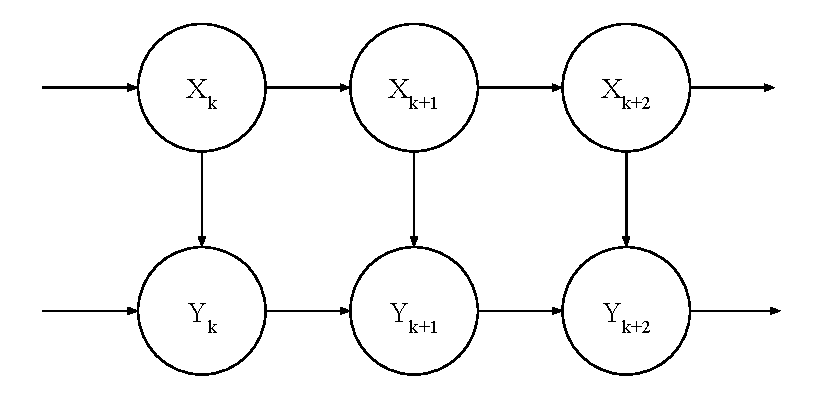
\includegraphics[width=0.75\textwidth]{hiddenmarkovmodel-1.pdf}
	\caption[Behavior of a hidden Markov model.]{Behavior of a hidden Markov model. The model goes through a sequence of hidden states ($X_k$) and produces an observable output at each state ($Y_k$).}
	\label{fig:hmm-1}
\end{figure}

A \ac{HMM} is a Markov chain where the state is not directly visible to an observer.
Instead, the \ac{HMM} outputs observations related to the underlying, hidden, chain.
The hidden chain is assumed to meet the Markov property.
A \ac{HMM} is pictured in Figure \ref{fig:hmm-1}
A \ac{HMM} can be described by the notation $\lambda = (\Pi, P, B)$, where $\Pi$ is the initial state distribution vector, $P$ is the matrix of state transition probabilities, and $B$ is a matrix describing the probability of observing an output given the hidden state.
Each row in $B$ maps each state in $X$ to a probability distribution for an observation from $Y$.
Let $y$ be some observation, where $y \in Y$, a finite set of discrete, possible observations.
$B$ then is a $|X|\times|Y|$ matrix where $B_{ij} = \Pr(Y=y_j|X=x_i)$, the probability of observing $y_j$ given the system is in some hidden state $x_i$.
This relationship is pictured in Figure \ref{fig:hmm-2}.
\nomenclature{$Y$}{A random variable or the set of observable states for a hidden Markov model}

\begin{figure}
	\centering
	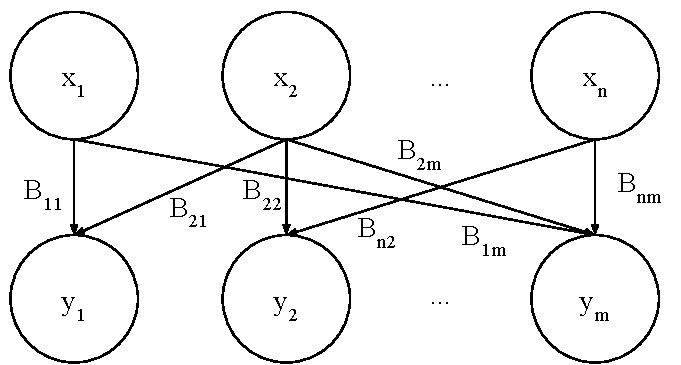
\includegraphics[width=0.75\textwidth]{hiddenmarkovmodel-2.pdf}
	\caption[Observable output of a hidden Markov model.]{Observable output of a hidden Markov model. Each state has a corresponding probability distribution for the observable outputs.}
	\label{fig:hmm-2}
\end{figure}

% Mention the joint probability distribution and cite that it also meets the markov property.
% That will be very helpful later I think.
A model where the state is a combination of $X$ and $Y$ from a \ac{HMM} is also a Markov model.
The state space for the new model, $Z$, is a set of tuples $Z = \{(X_0,Y_0), (X_0, Y_1), ... (X_1, Y_0), ... (X_n,Y_m)  \}$.
Where $\Pr(Z_k+1=(x_{k+1}, y_{k+1})|Z_k=(x_k, y_k)) = \Pr(Y_{k+1}=y_{k+1}|X_{k+1}=x_{k+1})\Pr(X_{k+1}=x_{k+1}|X_{k}=x_k)$.
Stated plainly, the probability that the joint model is some state $(x_{k+1},y_{k+1})$ is the probability that the hidden part of the model transitions to state $x_{k+1}$ and the observation for $x_{k+1}$ is $y_{k+1}$.
The probability distribution for the transition to the next state does not depend on the $y_k$ of the current state.

\section{Information Flow}

\subsection{Modal Logic}

A Kripke frame is a pair $<W,R>$\cite{french2006} such that $W$ is a set of possible worlds, where each world corresponds to a unique global state of the system.
Each element of $R$ describes a binary relationship for how the described system can move from world to world as events occur in the described system.
\nomenclature{$W$}{Set of worlds for a Kripke model or frame.}
\nomenclature{$R$}{Set of relations between worlds in a Kripke model or frame.}

In the case of a distributed system, a world could be described as one of the possible combinations of values of all boolean state variables $S=\{s_0, s_1, ... s_n\}$ in the system.
As execution occurs, messages, time, or events cause these variables to change.
Each change in boolean variables corresponds to a relationship in $R$\cite{Gehrke200565}.
Therefore, a world $w$ is one possible valuation of all the variables in $S$ and a transition from $w$ to another $w'$ (with its own valuation) can be noted as $wRw'$.
Without loss of generality, each relationship in $R$ must result in the change of at least one variable in $S$.
Additionally, the set of worlds is complete: every possible combination of state variable values is represented in the set of worlds.
No relationship in $R$ can lead to a world that does not exist.
\nomenclature{$S$}{Set of boolean state variables for a Kripke model.}

Additionally, we can define a set of valuation functions, $\mathbb{V}$.
Each function $V^i_{s_x}(w) \in \mathbb{V}$ describes the value observed by in a domain $D_i$ of a boolean state variable $s_x$ in some world $w$. 
If a valuation function for a particular state variable is not defined for an agent, the agent cannot determine the value of the state variable, and cannot determine the value of any logical statement based on the variable.
In the case of a distributed system, the valuation function concept is analogous to the isolation of memory for each agent.
For example, an agent $i$, cannot simply determine the value of a variable for agent $j$.
\nomenclature{$D_i$}{The domain of an agent or process $i$.}
\nomenclature{$\mathbb{V}$}{Set of valuation functions in a Kripke model.}
\nomenclature{$V$}{A valuation function.}

The combination of a Kripke Frame $< W,R >$ and a set of valuation functions $V$ is a Kripke model $K = \{W, R, V\}$, frequently known as a modal model.
The complete model describes all the possible worlds, the relation between those worlds and the information available in the domains of the system.
\nomenclature{$K$}{A Kripke model.}

Let $\varphi \in \Phi_0$ be an atomic proposition in a set of countably many propositions.
The set of well-formed formulas (wffs), as defined by the formulation rules in \ref{tab:axiomatic}, is the least set containing $\Phi_0$.
Additionally, we use the modal operator $\Box$ as an abbreviation for $\neg \Diamond \neg \varphi$.
The complete axiomatic system is outlined in \ref{tab:wffs}.
For the uninitiated, the modal box operator ($\Box$), ``it is necessary that'' states (in the case of $\Box \varphi$) ``in every world $w$, $\varphi$ is true.'' As its dual, the diamond operator ($\Diamond$) states ``there is a world where $\varphi$ is true.''
\nomenclature{$\varphi, \gamma, \psi$}{Well formed formulas.}
\nomenclature{$\Box \varphi$}{The modal ``it is necessary that'' operator.}
\nomenclature{$\Diamond \varphi$}{The modal ``it is possible that'' operator.}

\begin{table}[]
\small
\centering
\caption{Logical Statement Formulation Rules}
\begin{tabular}{r l}
1. & if $\varphi$ is a wff, so are $\neg \varphi$, $\Box \varphi$, and $\Diamond \varphi$. \\
2. & if $\varphi$ is a wff, so are $B_i \varphi$ and $\neg B_i \varphi$ \\
3. & if $\varphi$ is a wff, so are $T_{i,j} \varphi$ and $\neg T_{i,j} \varphi$ \\
4. & if $\varphi$ is a wff, so are $I_{i,j} \varphi$ and $\neg I_{i,j} \varphi$ \\
5. & if $\varphi$ and $\psi$ are both wff, so are $\varphi \wedge \psi$ \\
6. & if $\varphi$ and $\psi$ are both wff, so are $\varphi \vee \psi$ \\
\end{tabular}
\label{tab:wffs}
\end{table}

\begin{table}[!t]
\small
\centering
\caption{The Axiomatic System}
Definition of logical and modal operators (abbreviations) \\
\begin{tabular}{r l}
D1. & $\varphi \wedge \psi \equiv \neg ( \neg \varphi \vee \neg \psi)$\\
D2. & $\varphi \oplus \psi \equiv (\varphi \vee \psi) \wedge \neg(\varphi \wedge \psi)$ (exclusive or)\\
D3. & $\varphi \rightarrow \psi \equiv \neg \varphi \vee \psi $\\
D4. & $\varphi \leftrightarrow \psi \equiv (\varphi \rightarrow \psi) \wedge (\psi \rightarrow \varphi)$\\
D5. & $\Diamond \psi \equiv \exists w \in W : w \vdash \varphi $\\
D6. & $\Box \varphi \equiv \neg \Diamond \neg \varphi $\\
D7. & $B_i \varphi$ agent $i$ believes the truth of $\varphi$\\
D8. & $I_{i,j} \varphi$ agent $j$ informs $i$ that $\varphi \equiv \top$\\
D9. & $T_{i,j} \varphi$ agent $i$ trusts the report from $j$ about $\varphi$ \\
\end{tabular} \\~\\
Axioms \\
\begin{tabular}{r l}
P. & All the tautologies from the propositional calculus.\\
K. & $\Box (\varphi \rightarrow \psi) \rightarrow (\Box \varphi \rightarrow \Box \psi)$\\
M. & $\Box \varphi \rightarrow \varphi$\\
A1. & $\neg \Box \varphi \rightarrow \Box \neg \Box \varphi $\\
A2. & $\Diamond (\varphi \vee \psi) \rightarrow \Diamond \varphi \vee \Diamond \psi $\\
A3. & $\Box \varphi \wedge \Box \psi \rightarrow \Box (\varphi \wedge \psi)$ \\
B1. & $(B_i \varphi \wedge B_i (\varphi \rightarrow \psi )) \rightarrow B_i \psi$ \\
B2. & $\neg B_i \bot$\\
B3. & $B_i \varphi \rightarrow B_i B_i \varphi$ \\
B4. & $\neg B_i \varphi \rightarrow B_i \neg B_i \varphi$\\
I1. & $(I_{i,j} \varphi \wedge I_{i,j} (\varphi \rightarrow \psi )) \rightarrow I_{i,j} \psi$\\
I2. & $\neg I_{i,j} \bot$ \\
C1. & ($B_i I_{i,j} \varphi \wedge T_{i,j} \varphi) \rightarrow B_i \varphi$ \\
C2. & $T_{i,j} \varphi \equiv B_i T_{i,j} \varphi$ \\
\end{tabular} \\~\\
Rules of Inference \\
\begin{tabular}{r l}
R1. & From $\vdash \varphi$ and $\vdash \varphi \rightarrow \psi$ infer $\psi$ (Modus Ponens) \\
R2. & $\neg (\varphi \wedge \psi) \equiv (\neg \varphi \vee \neg \psi)$ (DeMorgan's)\\
R3. & From $\vdash \varphi$ infer $\vdash \Box \varphi$ (Generalization)\\
R4. & From $\vdash \varphi \equiv \psi$ infer $\vdash \Box \varphi \equiv \Box \psi$\\
R5. & From $\vdash \varphi \equiv \psi$ infer $\vdash T_{i,j} \varphi \equiv T_{i,j} \psi$\\
\end{tabular} \\
\label{tab:axiomatic}
\end{table}

\subsection{Non-Deducible (MSDND) Security}

In the domain of security, there are a wide variety of aspects worth protecting in every system.
These are grouped into the core security concepts of integrity, accessibility, and privacy.
Many traditional security approaches rely heavily on cryptography to provide privacy.
However, accidental information leakage can still occur, which compromises the privacy of the system.
For \ac{CPS}, the leakage is difficult to prevent.
Unlike their purely cyber counterparts, the actions taken by the physical components cannot be easily hidden from an observer.
For example, a plane changing altitude or a car turning or changing speed cannot be hidden from an observer.
Other, more complicated systems, like the power grid, have actions that are more difficult to observe. However, a well-motivated attacker can potentially collect critical information about the behavior of the cyber components with observations of the physical network\cite{Roth2012}.

Information flow security models are invaluable for assessing what information, if any, is leaked by either the cyber of physical components of the \ac{CPS}.
Many information flow security models, have been proposed, all based on similar concepts.
Typically, the models partition the system into two domains: the high-security domain and the low-security domain.
However, the MSDND security model allows the system to be partitioned into any number of domains.
The MSDND model has been used to describe how the STUXNET attack was able to hide its malicious behavior from the plant operators.
The MSDND security model is expressed using modal logic to determine what information in a domain is deducible to an observer in another domain.
The model exploits the possible worlds of modal logic to determine if there are worlds where the value of a logical atom is deducible by an agent outside the domain.

The MSDND security model can be used to determine what an agent in a distributed system can determine about another agent.
The exact specification of timing the distributed system becomes unnecessary as the modal model can express any combination of logical atoms in one of its worlds.\cite{Howser2012}\cite{STUXNET}\cite{Howser2013}

The MSDND security model can be expressed as follows\cite{STUXNET}.
Consider a pair of state variables $s_x$ and $s_y$ which may or may not be in the same security domain.
The value of $s_x$ and $s_y$ have a logical xor relationship: if $s_x$ is true, $s_y$ must be false.
Given an agent $i$ that does not have a valuation function for either of those two variables, the system is MSDND secure for the agent and pair of variables.
Written formally:

\begin{align}
MSDND = \exists w \in W : w \vdash \Box [ (s_x \vee s_y) \wedge \neg(s_x \wedge s_y) ] 
\nonumber \\ \wedge [ w \vDash ( \not \exists V_x^i (w) \wedge \not \exists V_y^i (w) ) ]
\end{align}

Of particular interest is the special case where $s_x$ and $s_y$ are relation on the same wff: $(s_x = \varphi$ and $s_y = \neg \varphi)$:

\begin{align}
MSDND = \exists w \in W : w \vdash \Box [ \varphi \oplus \neg \varphi ] 
\nonumber \\ \wedge [ w \vDash ( \not \exists V_\varphi^i(w)) ]
\end{align}

In a system where the above logical relationship holds, the agent $i$ cannot determine the value of $s_x$ or $s_y$. However, if the relationship does not hold, there is some world where the agent can determine the value of $s_x$ and $s_y$.

\subsection{BIT Logic}

% NEED CITATIONS FOR BIT LOGIC

\ac{BIT} was developed to formalize logic about belief and information transfer.
\ac{BIT} logic has typically been applied to distributed systems but has also played roles in \ac{CPS} security.
The operations of the \ac{BIT} logic allow formal definition of how entities pass information, and how they will act on the information passed to them.
\ac{BIT} logic utilizes several modal operators:

\begin{itemize}
\item $I_{i,j} \varphi$ defines the transfer of information directly from agent $j$ to an agent $i$. 
\item $T_{i,j} \varphi$ defines trust an agent $i$ has in a report from $j$ that $\varphi$ is true.
\item $B_i \varphi$ defines the belief that an agent $i$ has about $\varphi$. The actual value of $\varphi$ is irrelevant: the agent $i$ believes it to be true.
\end{itemize}
\nomenclature{$I_{i,j}$}{The modal information transfer operator.}
\nomenclature{$T_{i,j}$}{The modal trust operator.}
\nomenclature{$B_i$}{The modal belief operator.}

These operators allow reasoning about information transfer between entities.
In the context of a distributed system, these operators allow the division of the actual state held by some agent $i$ to what some other agent $j$ believes is agent $i$'s state.

\section{Explicit Congestion Notification}

\ac{ECN} is a technique for managing congestion in IP networks. 
When an \ac{ECN} capable network device detects congestion, it can drop the packets, or it can signal senders using flags in the packet headers that the network is congested.
For a TCP application, the result of the dropped packets causes the slow-start congestion control strategy to reduce the rate packets are sent.
A more advanced implementation, using \ac{ECN}, sets specific bits in the TCP header to indicate congestion.
By using \ac{ECN}, TCP connections can reduce their transmission rate without re-transmitting packets.

UDP applications have not typically utilized \ac{ECN}.
Although the \ac{ECN} standard has flags in the IPv4 header, access to the IPv4 header is not possible on most systems.
Furthermore, there is not a ``one size fits all'' solution to congestion in UDP algorithms.

\subsection{Random Early Detection (RED)}
The \ac{RED} queuing algorithm is a popular queuing algorithm for switches and routers.
It uses a probabilistic model and an \ac{EWMA} to determine if the average queue size exceeds predefined values.
The values are used to identify potential congestion and manage it.
Congestion identification is accomplished by determining the average size of the queue, and then probabilistically dropping packets to maintain the size of the queue.
In \ac{RED}, when the average queue size, $avg$, exceeds a minimum threshold ($min_{th}$), but is less than a maximum threshold ($max_{th}$), new packets arriving at the queue may be ``marked''.
The probability a packet is marked is based on the following relation between $p_{b}$ and $p_{a}$ where $p_{a}$ is the final probability a packet will be marked.

\begin{equation}
p_{b} = max_p (avg - min_{th}) / (max_{th}-min_{th})
\end{equation}
\begin{equation}
p_{a} = p_{b} / (1-count * p_b)
\end{equation}

Where $max_p$ is the maximum probability a packet will be marked when the queue size is between $min_{th}$ and $max_{th}$ and $count$ is the number of packets since the last marked packet.
With \ac{RED}, the probability a packet is marked varies linearly with the average queue size, and as a function of the time since the last packet was marked.
If $avg$ is greater than $max_{th}$, the probability of marking trends toward one as the average queue size approaches $2*max_{th}$.
In the event the queue fills completely, the \ac{RED} queue operates as a drop-tail queue.
In a simple implementation of the \ac{RED} algorithm, marked packets are dropped.

\section{Distributed Grid Intelligence (DGI)}

The DGI is a smart grid operating system that organizes and coordinates power electronics.
It also negotiates contracts to deliver power to devices and regions that cannot effectively facilitate their needs.
DGI leverages common distributed algorithms to control the power grid, making it an attractive target for modeling a distributed system.
Algorithms employed by the \ac{DGI} and grouped into modules, work together to migrate power from areas of excess supply to excess demand.

DGI utilizes several modules to manage a distributed smart-grid system.
Group management, which is our main focus, implements a leader election algorithm to discover which processes are reachable within the cyber domain.
Other modules provide additional functionality, such as collecting global snapshots, negotiating the migrations, and giving commands to physical components.

DGI is a real-time system; certain actions (and reactions) involving power system components need to be completed within a pre-specified time frame to keep the system stable.
It uses a round robin schedule where each module is given a predetermined window of execution which it may use to perform its duties.
When a module's round ends, the next module in the line is allowed to execute. 

The DGI uses the leader election algorithm, ``Invitation Election Algorithm,'' written by Garcia-Molina\cite{INVITATIONELECTION}.
The algorithm provides a robust election procedure which allows for transient partitions.
Transient partitions are formed when a faulty link inside a group of processes causes the group to divide temporarily.
The transient partitions merge when the link becomes more reliable.

\subsection{Real Time}
Real-time requirements were designed to enforce a tight upper bound on the amount of time used creating groups, discovering peers, collecting the global state, and performing migrations.

To enforce these bounds, the real-time DGI has distinct phases which modules were allowed to use for all processing.
Each module was given a round with a specific amount of processor time allocated to the module.
Modules used the allocated time to complete any tasks they had prepared.
When the allotted time was up, the scheduler changed context to the next module.
This interaction is illustrated in Figure \ref{fig:REALTIMESCHEDULER}

\begin{figure}[!h]
\centering
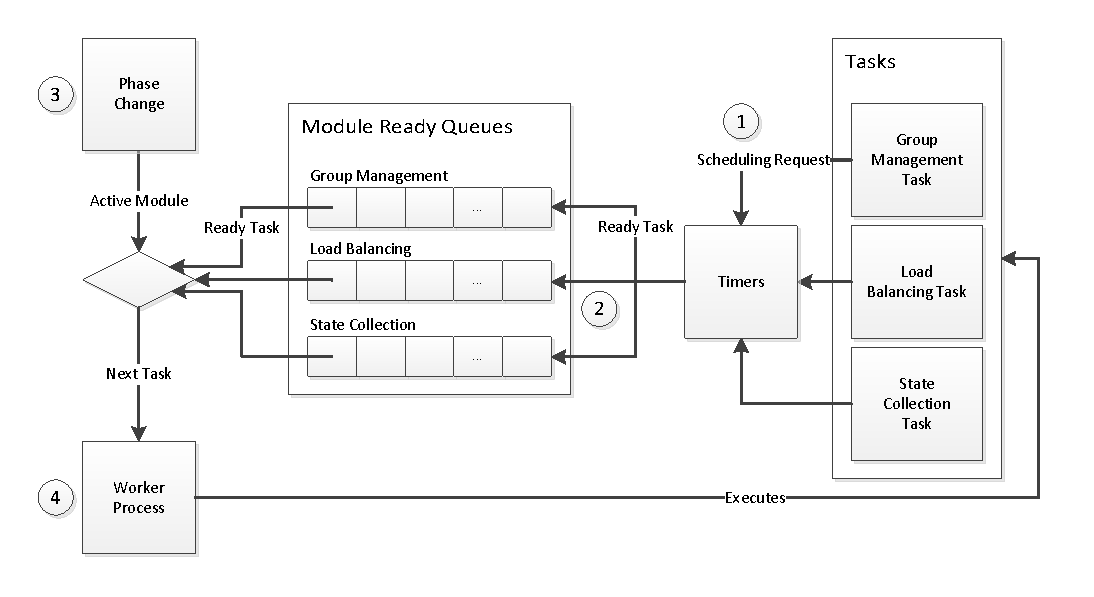
\includegraphics[width=1.0\textwidth]{RealTimeScheduler.pdf}
\captionsetup{singlelinecheck=off}
\caption[Real Time Scheduler]{The real time scheduler used a round robin approach to allot execution time to modules. 
\begin{enumerate}
    \item Modules requested a task be executed by specifying a time in the future to execute the task.
          A timer was set to count down to the specified moment.
           Modules could place tasks immediately into the ready queue if the task could be executed immediately.
    \item When the timer expires, the task is placed into the ready queue.
    \item Modules were assigned periods of execution (called phases) of a predetermined length.
          After the specified amount of time had passed, the module's phase ends and the next module in the schedule began to execute.
    \item The worker selected the next ready task for the active module from the ready queue and executed it.
          These tasks could also schedule other tasks to be run in the future.
\end{enumerate}
}
\label{fig:REALTIMESCHEDULER}
\end{figure}

Modules informed the scheduler of tasks they wish to perform.
The tasks could be scheduled for some point in the future, or scheduled to be executed immediately.
When a task became ready, it was inserted into a ready queue for the module which scheduled the task.

When the module's phase was active, tasks were pulled from the ready queue and executed.
When the phase was complete, the scheduler stopped pulling tasks from the previous module's queue and began pulling from the next module's queue.

Using a round robin scheduler allowed enforcement of an upper bound on message delay.
Modules had a specific amount of processing time allotted.
Modules with messages that invoked responses typically required the responses to be received within the same phase.
Round numbers enforced that the message was sent within the same phase.

Modules were designed and allotted time to allow for parameters such as maximum query/response time (based on the latency between communicating processes).
Modules using the scheduler had an upper-bound in response time before messages were considered lost.

\subsection{Group Management Algorithm}

The DGI uses the leader election algorithm, ``Invitation Election Algorithm,'' written by Garcia-Molina\cite{INVITATIONELECTION}.
Originally published in 1982, the algorithm provides a robust election procedure that allows for transient partitions.
Transient partitions are formed when a faulty link between two or more clusters of \ac{DGI} causes the groups to divide temporarily.
These transient partitions merge when the link becomes more reliable.
The election algorithm allows for failures that disconnect two distinct sub-networks.
These sub-networks are fully connected, but connectivity between the two sub-networks is limited by an unreliable link.

Since Garcia-Molina's original publication \cite{INVITATIONELECTION}, a large number of election algorithms have been created. 
Each algorithm is designed to be well-suited the problem space where it is used.
Specialized algorithms exist for wireless sensor networks\cite{LE-WSN-1}\cite{LE-WSN-2}, detecting failures in certain circumstances\cite{LE-SPECIALCIRCUMSTANCES-1}\cite{LE-SPECIALCIRCUMSTANCES-2}, and of course, transient partitions.
Work on leader elections has been incorporated into a variety of distributed frameworks: Isis\cite{ISISTOOLKIT}, Horus\cite{HORUSTOOLKIT}, Totem\cite{TOTEMTOOLKIT}, Transis\cite{TRANSISTOOLKIT}, and Spread\cite{SPREADTOOLKIT} all have methods for creating groups.
Despite the broad range of work, the fundamentals of leader election are consistent
across all work.
Processes arrive at a consensus of a single peer that coordinates the group.
Processes that fail are detected and removed from the group. 

The elected leader is responsible for making work assignments, and identifying and merging with other coordinators when they are found, as well as maintaining an up-to-date list of peers for the members of his group. 
Group members monitor the group leader by periodically checking if the group leader is still alive by sending a message. 
If the leader fails to respond, the querying nodes will enter a recovery state and operate alone until
they can identify another coordinator.
Therefore, a leader and each of the members maintains a set of processes which are currently reachable, a subset of all known processes in the system.

Leader election can also be classified as a failure detector\cite{LEADERELECTIONEVAL}.
Failure detectors are algorithms which detect the failure of processes within a system; they maintain a list of processes that they suspect have crashed.
This informal description gives the failure detector strong ties to the leader election process. 
The group management module maintains a list of suspected processes which can be determined from the set of all processes and the current membership.

The leader and the members have separate roles to play in the failure detection process.
Leaders use a periodic search to locate other leaders to merge groups.
This query also serves to detect failures within the system.
The member sends a query to its leader.
The member will only suspect the leader and not the other processes in their group.

Using a leader election algorithm allows the \ac{FREEDM} system to autonomously reconfigure in the event of a failure.
Cyber components are tightly coupled with the physical components, and reaction to faults is not limited to faults originating in the cyber domain.
Processes automatically react to crash-stop failures, network issues, and power system faults.
The automatic reconfiguration allows processes to react immediately to issues, faster than a human operator, without relying on a central configuration point.
However, it is important the configuration a leader election algorithm supplies is one where the system can do viable work without causing physical faults like voltage collapse or blackouts\cite{HARINI}.

A state machine for the election portion of the election algorithm is shown in Figure \ref{fig:statemachine}.
In the normal state, the election algorithm regularly searches for other coordinators.
When another coordinator is identified, all other processes will yield to their future coordinator.
The method of selecting which process becomes the coordinator of the new group differentiates the modified algorithm from other approaches.

\subsection{Power Management}

We utilized the load balancing algorithm from \cite{LOADBALANCING}.
The load balancing algorithm performs work by managing power devices with a sequence of migrations\cite{HILTESTBED}.
In each migration, a sequence of message exchanges identify processes whose power devices are not sufficient to meet their local demand and other processes supply them with power by utilizing a shared bus.
First, processes that cannot meet their demand announce their need to all other processes.
Processes with devices that exceed their demand offer their power to processes that announced their need.
These processes perform a three-way handshake.
At the end of the handshake, the two processes have issued commands to their attached devices to supply power from the shared bus and to draw power from the shared bus.
An example of how the power system is affected by migrations is depicted in Figure \ref{fig:good-migrations}.
In the chart, processes with net generation (generation $>$ 0) share power with processes with excess loads.
As processes with excess loads are satisfied, both supply and demand processes trend toward 0 net generation.

\begin{figure}
\centering
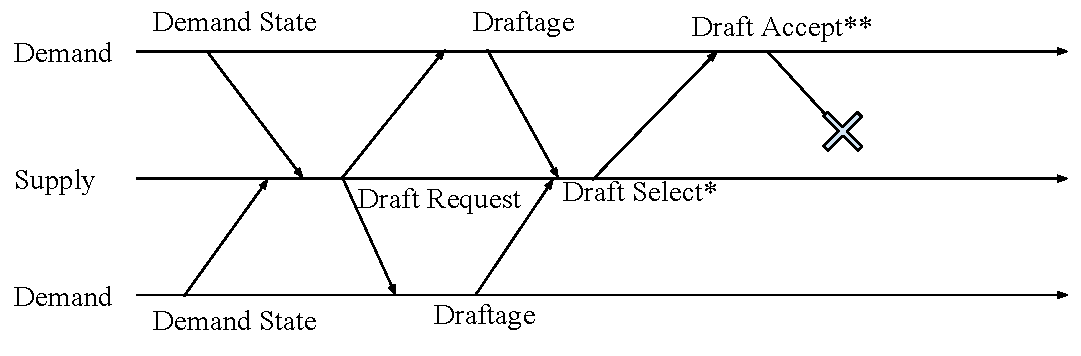
\includegraphics[width=0.95\textwidth]{FailedMigration1}
\caption{Example of a failed migration. (*) and (**) mark moments when power devices change state to complete the physical component of the migration. In this scenario, the message confirming the demand side made the physical is lost, leaving the supply node uncertain.}
\label{fig:failed-migration-1}
\end{figure}

\begin{figure}
\centering
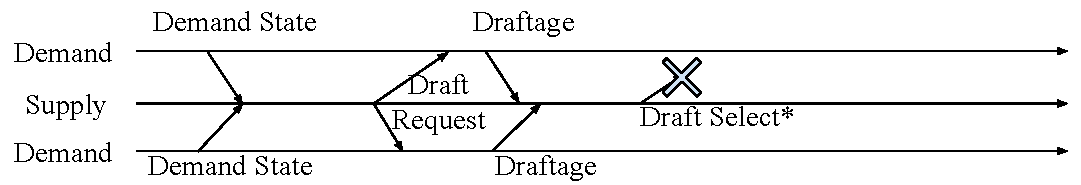
\includegraphics[width=0.95\textwidth]{FailedMigration2}
\caption{Example of a failed migration. (*) marks a moment when power devices change state to complete the physical component of the migration. In this scenario, the supply process changes its device state, but the demand process does not.}
\label{fig:failed-migration-2}
\end{figure}

\begin{figure}
\centering
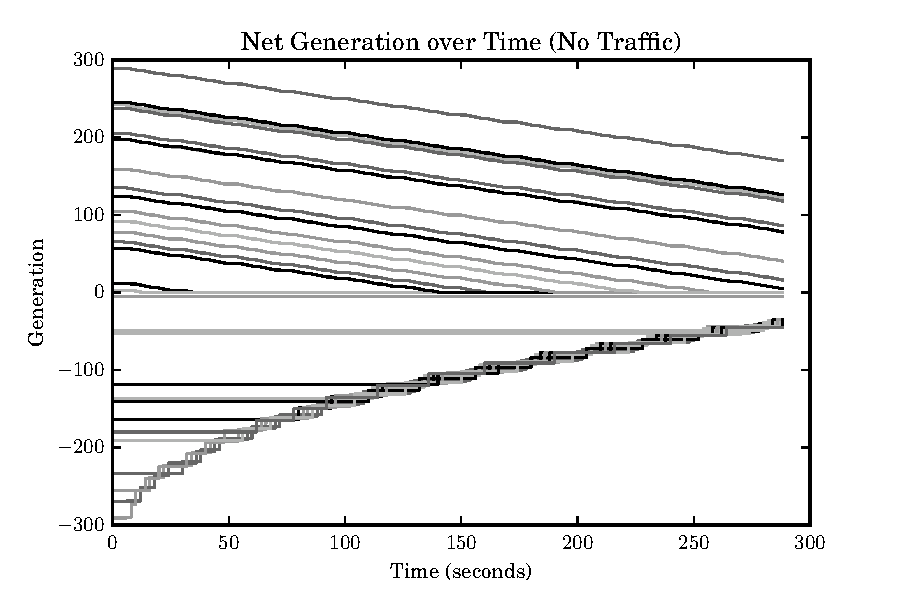
\includegraphics[width=0.75\textwidth]{c-migrations-no-traffic-all}
\caption{Each migration consumes excess generation capability and removes excess demand.}
\label{fig:good-migrations}
\end{figure}

The \ac{DGI} algorithms can tolerate packet loss and is implemented using UDP to pass messages between \ac{DGI} processes.
Effects of packet loss on the \ac{DGI}'s group management module have been explored in \cite{CRITIS2012} and \cite{JOURNAL}.
The load balancing algorithm can tolerate some message loss, but lost messages can cause migrations to only partially complete, which can cause instability in the physical network.
A failed migration is diagrammed in Figures \ref{fig:failed-migration-1} and \ref{fig:failed-migration-2}.
With the power migration algorithm, uncompensated actions may occur in the power system.
These actions can eventually lead to power instability through issues such as voltage collapse.
Additionally, the supply process may not always be certain if the second half of the action was completed or not.
If the ``Draft Accept'' message does not arrive from the demand process, the supply process cannot be certain of if its ``Draft Select'' message was received.
If the supply process takes action to compensate by reversing the migration and the confirmation arrives later, the system will also be driven towards instability because another process completed an uncompensated action.
Processes could confirm the number of failed migrations with a state collection technique.
It is, therefore, desirable to manage the processes to minimize the number of failed migrations.



% RESULTS
%   - Show the unbounded Queue Graph and the mess it makes of LB and GM
%   - Show soft ECVN allows more work to be done, possibly at the cost of accumulating K.
%   - Shwo that HARD ecn allows the best operation -- work gets done and less K is accumlated.

\chapter{Conclusion}

This work presented a new approach for predicting the behavior of a real-time distributed system under omission failure conditions. By using a continuous time Markov chain, a variety of insights can be gathered about the system, including observations such as how long a particular configuration will be stable, and the behavior of the system in the long run.  The Markov results will be used  to make better real time schedules to better react to the network faults we plan on introducing to our test beds. The primary concern are scenarios in which the cyber controller attempts to make physical components which are not connected in the physical network interact, and scenarios where a fault in the cyber network causes the paired events (where two physical controllers change to accomplish some transaction or exchange) to only be partially executed. For example, in the DGI load balancing scheme, a node in a supply state injects a quantum of power into the physical network, but the node in the demand state does not change to accept it. These errors, which are the primary focus of this work could cause instability if a sufficient number of these failed exchanges occur. In \cite{HARINI}, Choudhari et. al. show that failed transactions can create a scenario where the frequency of a power system could become unstable. 

Moving forward, we have identified these areas as targets for improving the research done and creating new contributions.

\section{Time between reconfigurations}

 The rate that the system should reconfigure is a function of the maximum number of failed migrations that the system can handle before becoming unstable, the time it takes to write to the channel and the time it takes process messages. The amount of time in group can also be a consideration for which algorithm to select based on the needed amount of time to perform its work. Group Management can be used as a critical component in a real-time distributed system to manage the number of lost messages and as a consequence, the number of failed migrations in a CPS. It is critical to understand how frequently nodes enter and exit the group based on lost messages and how many migrations fail as a consequence of those messages. This area is deficient because it is strongly coupled to the interactions with the physical component: we must understand how the cyber configuration and physical changes made by that configuration can affect the system, and establish when reconfigurations should occur to keep the system stable. To correct this, we hope to develop a mathematical relationship between the stability of the group, and the physical management functionality of the CPS.

\section{Correctness of an Installed Configuration}

 The work presented in this document is probabilistic: the results of a leader election are random and based only on responses arriving with in a specified period of time. Other factors can affect what configurations can be installed such as trust in the parties in the group, the underlying physical topology, and the reliability of the peers in that group. We hope to develop guarantees on the properties of a configuration that protect the physical topology and the members of the group. These guarantees would also allow processes to better police the configurations they are installed in, in order to protect the system from malicious nodes.

\section{Accuracy of The Model}

We recognize that the model presented thus far does not have ideal accuracy. We expect to be able to further refine the model and the algorithms and formulas for generating the model. There are some features of the behavior of the DGI which are not completely encapsulated in the model. Additionally, the way models are specified can be generalized to support more systems of similar design. As part of this work however, we must remember modeling distributed systems is extremely difficult and while the increase in accuracy is desirable it is not a critical goal.

\section{Scope of the Model}

The models presented in this work focus only on the leader election component of a dynamically configured CPS. Additional work would incorporate additional components of the DGI system into the models for a more complete picture of the behavior of the system during failures. We will consider the correctness of the incorporated algorithms, how omission failures can violate that correctness, and what restrictions we can place on the configuration and operation of DGIs in order to protect the entire system during failures. To do this, we will expand the analysis performed here to incorporate algorithms such as state collection and load balancing and define metrics to quantify their behavior during omission failures. This thrust will pair with the correctness and time between reconfigurations: different algorithms will have different amounts of failure that can be allowed before reconfiguration is necessary.

\section{Deliverables}

Therefore, moving forward, we will expand the models we have presented here to include more of the properties of the complete CPS. This model will allow us to better understand what effects the group behavior has on the CPS. Using this, we can establish invariants which allow us to ensure the correctness of a CPS by providing assertions which will not be broken during execution. Creating these invariants will allow us to improve the development of CPSs, especially in their dynamic configuration, which is an area with limited development. These invariants also allow us to create an assertion of correctness which can be validated, during runtime, to ensure the system maintains its stability. We will continue to create and validate models of the CPS against simulations and actual hardware. As we do so we will construct invariants that describe the correct behavior of the groups to ensure safe operation. In addition to the existing conference paper \cite{CRITIS2012}, we have prepared a journal paper with the new work in this document. 
%\lipsum[1-20]% to test page spacing
%\end{ThesisBackMatter}
\end{ThesisBody}

\begin{ThesisAppendix}{three}
%\section{SRC Protocol}

The following the psuedocode for the SRC protocol, which is a sequenced reliabile protocol. Messages are delivered before a prespecified deadline. If the message is not delivered before the deadline the message is no longer sent and the next message (if it is not expired) is delivered instead. The scheme is a modified send-and-wait scheme so at most one message is being delivered at a time. This is,a version with unbounded
sequence numbers. The implementation available with the FREEDM source code is modified to allow for bounded sequence numbers.

\begin{algorithmic}

\State $inseqno \gets 0$
\State $outseqno \gets 1$
\State $outqueue \gets []$
\State $kill \gets null$
\State $lastack \gets 0$

\Function{Receive}{msg}
    \If {$msg.type = MSG$}
        \If {$msg.seqno = inseqno+1$}
            \State $SendAck(msg.seqno)$
            \State $inseqno \gets inseqno + 1$
        \ElsIf {$msg.seqno > inseqno$ and $msg.kill \neq null$ and $msg.kill 
\leq inseqno$}
            \State $SendAck(msg.seqno)$
            \State $inseqno \gets msg.seqno + 1$
        \Else
            \State $SendAck(inseqno)$
        \EndIf
    \ElsIf {$msg.type = ACK$}
        \If {$msg.seqno = outqueue.front.seqno$}
            \State $outqueue.pop()$
            \State $kill \gets null$
            \State $lastack \gets msg.seqno$
            \State $Write(outqueue.front,kill)$
        \Else
            \State $Write(outqueue.front,kill)$
        \EndIf
    \EndIf
\EndFunction

\Function{Send}{msg}
    \State $msg.seqno \gets outseqno$
    \State $outseqno \gets outseqno+1$
    \State $outqueue.push(msg)$
    \If {$outqueue.size = 0$}
        \State $Write(outqueue.front,kill)$
    \EndIf
\EndFunction

\Function{Resend}{}
    \While{$outqueue.size \geq 0$ and $outqueue.front.expired$}
        \State $outqueue.pop()$
        \State $kill \gets lastack$
    \EndWhile
    \If {$outqueue.size \geq 0$}
        \State $Write(outqueue.front,kill)$    
    \EndIf
\EndFunction

\end{algorithmic}

\section{SUC Protocol}

The following is the psuedocode for the SUC protocol which is a sequenced unreliable protocol. Messages are ordered, but delivery is not guaranteed. The protocol is a modified sliding window protocol so several messages are sent for delivery at the same time. If a message with a higher sequence number is recieved, messages with lower sequence numbers are considered lost (unless they've already been delivered) and if they arrive later, out of order, they are discarded.

\begin{algorithmic}

\State $inseqno \gets 0$
\State $outseqno \gets 0$
\State $outqueue \gets []$

\Function{Receive}{msg}
    \If {$msg.type = MSG$}
        \If {$msg.seqno > inseqno$}
            \State $SendAck(msg.seqno)$
            \State $inseqno \gets msg.seqno$
        \Else
            \State $SendAck(inseqno)$
        \EndIf
    \ElsIf {$msg.type = ACK$}
        \State $popped \gets 0$
        \If {$msg.seqno \leq outqueue.front.seqno$}
            \State $outqueue.pop()$
            \State $popped \gets popped+1$
        \EndIf
        \For{$i = WindowSize-popped \to min(WindowSize-1,outqueue.size)$}
            \State $Write(outqueue[i])$
        \EndFor
    \EndIf
\EndFunction

\Function{Send}{msg}
    \State $msg.seqno \gets outseqno$
    \State $outseqno \gets outseqno+1$
    \State $outqueue.push(msg)$
    \If {$outqueue.size \leq WindowSize$}
        \State $Write(msg)$
    \EndIf
\EndFunction

\Function{Resend}{}
    \For{$i = 0 \to min(WindowSize-1,outqueue.size)$}
        \State $Write(outqueue[i])$
    \EndFor
\EndFunction

\end{algorithmic}

\section{Leader Election}

The following is the psuedocode for Garcia-Molina's leader election algorith orginially published in CITE. Leaders are responsible for detecting the failure of each of the members and reporting it to the rest of the group. Members detect the failure of the leader and perform elections to combine groups.

\begin{algorithmic}

\State $AllNodes \gets \{ 1, 2, ..., N \}$
\State $Coordinators \gets \emptyset$
\State $UpNodes \gets { Me }$
\State $State \gets Normal$
\State $Coordinator \gets Me$
\State $Responses \gets \emptyset$
\State $Counter \gets$ A random initial identifier
\State $GroupID \gets (Me,Counter)$

\State

\Function{Check}{}
    \State This function is called periodically by the leader
    \If {$State = Normal$ and $Coordinator \gets Me$}
        \State $Responses \gets \emptyset$
        \State $TempSet \gets \emptyset$
        \For {$j = (AllNodes - \{Me\})$}
            \State $AreYouCoordinator(j)$
            \State $TempSet \gets TempSet \cup j$
        \EndFor
        \State Nodes which respond "Yes" to $AreYouCoordinator$ are put into 
the $Responses$ set. When all nodes have responded or after 
$Timeout(CheckTimeout)$, Nodes that do not respond are removed from UpNodes and 
execution continues
        \State $UpNodes \gets (TempSet-Responses) \cup {Me}$
        \If {$Responses = \emptyset$}
            \Return
        \EndIf
        \State $p \gets \max(Responses)$
        \If $Me < P$
            \State Wait time proportional to p-i
        \EndIf
        \Call{Merge}{Responses}
    \EndIf
    \State The next call to this is after Timeout(CheckTimeout)
\EndFunction

\State

\Function{Timeout}{}
    \State This function is called periodically by the group members
    \If {$Coordinator = Me$}
        \Return
    \Else
        \Call{AreYouThere}{Coordinator,GroupID,Me}
        \If{Response is No or after $Timeout(TimeoutTimeout)$}
            \Call{Recovery}{}
        \EndIf
    \EndIf
    \State The next call to this is after Timeout(TimeoutTimeout)
\EndFunction

\State

\Function{Merge}{Coordinators}
    \State This function invites all coordinators in Coordinators to join a 
group led by Me
    \State $State \gets Election$
    \State Stop work
    \State $Counter \gets Counter+1$
    \State $GroupID \gets (Me,Counter)$
    \State $Coordinator \gets Me$
    \State $TempSet \gets UpNodes - {Me}$
    \State $UpNodes \gets \emptyset$
    \For {$j \in Coordinators$}
        \Call{Invite}{j,Coordinator,GroupID}
    \EndFor
    \For {$j \in TempSet$}
        \Call{Invite}{j,Coordinator,GroupID}
    \EndFor
    \State Wait for $Timeout(InviteTimeout)$, Nodes that accept the invite are 
added to UpNodes
    \State $State \gets Reorganization$
    \For {$j \in UpNodes$}
        \Call{Ready}{j,Coordinator,GroupID,UpNodes}
    \EndFor
    \State $State \gets Normal$
\EndFunction

\State

\Function{ReceiveReady}{Sender,Leader, Identifier, Peers}
    \If {$State = Reorganization$ and $GroupID = Identifier$}
        \State $UpNodes \gets Peers$
        \State $State \gets Normal$      
    \EndIf
\EndFunction

\State

\Function{ReceiveAreYouCoordinator}{Sender}
    \If {$State = Normal$ and $Coordinator = Me$}
        \State Respond Yes
    \Else
        \State Respond No
    \EndIf
\EndFunction

\State

\Function{ReceiveAreYouThere}{Sender, Identifier}
    \If {$GroupID = Identifier$ and $Coordinator = Me$ and $Sender \in UpNodes$}
        \State Respond Yes
    \Else
        \State Respond No
    \EndIf
\EndFunction

\State

\Function{ReceiveInvitation}{Sender,Leader,Identifier}
    \If {$State \neq Normal$}
        \Return
    \EndIf
    \State Stop Work
    \State $Temp \gets Coordinator$
    \State $TempSet \gets UpNodes$
    \State $State \gets Election$
    \State $Coordinator \gets Leader$
    \State $GroupID \gets Identifier$
    \If {$Temp = Me$}
        \State Forward invite to old group members
        \For $j \in TempSet$
            \State $Invite(j,Coordinator,GroupID)$
        \EndFor
    \EndIf
    \State $Accept(Coordinator,GroupID)$
    \State $State \gets Reorganization$
    \If {$Timeout(ReadyTimeout)$ expires before $Ready$ is recieved}
        \State $Recovery()$
    \EndIf
\EndFunction

\State

\Function{ReceiveAccept}{Sender,Leader,Identifier}
    \If {$State \gets Election$ and $GroupID = Identifier$ and $Coordinator = 
Leader$}
        \State $UpNodes \gets UpNodes \cup {Sender}$
    \EndIf
\EndFunction

\State

\Function{Recovery}{}
    \State $State \gets Election$
    \State Stop Work
    \State $Counter \gets Counter + 1$
    \State $GroupID \gets (Me,Counter)$
    \State $Coordinator \gets Me$
    \State $UpNodes \gets {Me}$
    \State $State \gets Reorganization$
    \State $State \gets Normal$
\EndFunction

\end{algorithmic}
%\chapter{Characteristic Length Scales}
\label{sec:lengths}
%This table lists lengths used in the dissertation.

\captionsetup[table]{list=no}
%\begin{center}
\begin{table} % for label and caption purposes
%\begin{tabular}{|l|l|l|} % table runs off page
%\begin{tabular}{|l|l|p{7cm}|} % center column too large
\caption{Length scales used in this dissertation}
\begin{tabular}{|l|p{4cm}|p{8.5cm}|}
%\begin{tabular*}{0.75\textwidth}{|l|l|l|}{@{\extracolsep{\fill}} | c | c | c | }
\hline Symbol & Name & Description \\ \hline
$\lambda$ & wavelength & Wavelength of incident light \\ 
$L$ &  system length & Length of waveguide along direction of propagation ($z$-axis) \\ 
$W$ & system width & Dimension of waveguide perpendicular to direction of propagation ($y$-axis) \\
$L_{\phi}$ & phase coherence length & Length over which phase remains coherent. Equivalent to $L_{inelastic}$\cite{1988_Stone,1986_Imry}. Applicable only to electron transport. \\
$L_D$ & path length & How far a particle (i.e. ray optics) travels in the media in ballistic and diffusive regimes \\
$\ell_{scat}$ & scattering length & Average distance between scattering events. Often referred to as $\ell_{mfp}$ (mean free path) or the inelastic length\cite{1984_John_prl}, or extinction length\cite{1999_van_Tiggelen}. \\ 
$\ell_{tmfp}$ & transport mean free path & Average distance over which phase and direction are randomized.  $\ell_{tmfp} = \frac{\ell_{scat}}{1-\langle cos\ \theta \rangle}$. Sometimes referred to as elastic mfp\cite{1991_John}. % page 34, col 2
Measured with respect to $L$. \\ 
$\xi$ & localization length & Probability of diffusive path forming loop is 1. $\xi~=~N~\ell_{tmfp}$. Measured with respect to $L$. \\ 
$\ell_{a,g}$ & ballistic absorption/gain length & Average distance over which intensity decreases by two/increases by two. \\
$\xi_{a,g}$ & absorption/gain length & How far, on average, a particle travels in the diffusive regime before being absorbed (or doubled), measured with respect to path length $L_D$ in the diffusive regime \\ 
$z_p$ & penetration depth & Applies to diffusive regime only. $z_p \approx \ell_{tmfp}$ \\ 
\hline
\end{tabular}

\ \\ 

\label{tabl:lengths}
\end{table}
%\end{center}
All length scales (except $\lambda$) are normalized by wavelength. % lengths can be converted to equivalent times by $\ell = c t$
%\captionsetup[table]{list=yes} % referenced in introduction
%\chapter{Transmission Derivation}

This is an expanded version of the analysis performed for Fig.~\ref{fig:energydistrib}

\begin{equation}
T = T(\omega, x_o) = \frac{(\exp(-\frac{L}{\xi}))^2}{ 
(\omega-\omega _o)^2 + (\exp(-\frac{L}{\xi})\frac{1}{2}\exp(\frac{\mid L-2 x_o \mid}{\xi}))^2 }
\label{fig:appendixtransmission}
\end{equation}
Where we have appoximated cosh() as $\frac{1}{2}\exp()$. 

From the behavior of transmission in media with defects and centers of localizaiton, we see two cases when on a resonant frequency:  either the defect is in the first half of the sample.%, (\ref{fig:cononicaldefectpositions}, plot 1).

\begin{equation}
{\cal E}(x) = \left\{ 
\begin{array}{l l}
  A \exp\left(\frac{2 (x-x_o)}{\xi}\right) & \quad 0 < x < x_o \\
  B \exp\left(-\frac{2 (x-x_o)}{\xi}\right) & \quad x_o < x < L\\
\end{array} \right.
\label{fig:left}
\end{equation}

or it is in the second half of the sample.%, (\ref{fig:cononicaldefectpositions}, plot 2).
\begin{equation}
{\cal E}(x) = \left\{ 
\begin{array}{l l}
 A \exp\left(-\frac{2 x}{\xi}\right) & \quad 0 < x < L-2 x_o \\
 B \exp\left(\frac{2 (x-x_o)}{\xi}\right) & \quad L-2 x_o < x < x_o \\
 C \exp\left(-\frac{2 (x-x_o)}{\xi}\right) & \quad x_o < x < L \\
\end{array} \right.
\label{fig:right}
\end{equation}

With either case, we see three distinct regions when the frequency is not on resonance but prior to the pure exponential decay regimes. %(\ref{fig:cononicaldefectpositions}, plot 3):
\begin{equation}
{\cal E}(x) = \left\{ 
\begin{array}{l l}
y_1 = A \exp\left(-\frac{2 x}{\xi}\right)   & \quad 0 < x < x_1  \\
y_2 = B \exp\left(\frac{2 (x-x_o)}{\xi}\right) & \quad x_1 < x < x_o  \\
y_3 = C \exp\left(-\frac{2 (x-x_o)}{\xi}\right) & \quad  x_o < x < L \\
\end{array} \right.
\label{fig:startingequations}
\end{equation}
Where $x_1$ is the turning point.

\begin{comment}
%% pictures were removed, causes a problem during compile (?)
\begin{figure}
\vskip -0.5cm
\centerline{
\scalebox{0.5}{\includegraphics{pictures/transmission_derivation_14_LR}}
\scalebox{0.5}{\includegraphics{pictures/transmission_derivation_34_LR}}
\scalebox{0.5}{\includegraphics{pictures/transmission_derivation_off_res_LR}}
}
\vskip -0.5cm
\caption{Log of energy versus position sketches for a center of localization in the first half (left), Eq.~\ref{fig:left}; and second half (center), Eq.~\ref{fig:right}. The turning point in the center plot is $L-2 x_o$. The right sketch is off-resonance but prior to pure exponential decay, which applies to any center of localization position, as described by Eq.~\ref{fig:startingequations}. The turning point in the right plot from the initial exponential decay to growth varies depending how far off resonance one is. We call this $x_1$}
\label{fig:cononicaldefectpositions}
\end{figure}
\end{comment}

From the off-resonance Eq.~\ref{fig:startingequations}, we apply boundry conditions to determine the coefficients in passive systems. We take gain into account and make corrections later.

At $x=0$ then $y_1=4$, giving $A=4$. Thus
\begin{equation}
\boxed{y_1 = 4 \exp\left(-\frac{2 x}{\xi}\right)}   \quad \quad \quad 0 < x < L-2 x_o 
\end{equation}

At $x=L$, $y_3=T$. Solve for C,
\begin{equation}
C=T \exp\left(\frac{2(L-x_o)}{\xi}\right)
\end{equation}
plug back in,
\begin{equation}
y_3 = T \exp\left(\frac{2(L-x_o)}{\xi}) \exp(-\frac{2 (x-x_o)}{\xi}\right)  \quad \quad \quad  x_o < x < L
\end{equation}
simplify to get
\begin{equation}
\boxed{y_3 = T \exp\left(-\frac{2(x-L)}{\xi}\right)}  \quad \quad \quad  x_o < x < L
\end{equation}
at $x_o$, $y_2 = y_3$
\begin{equation}
B \exp\left(\frac{2 (x_o-x_o)}{\xi}\right) = B = T \exp\left(-\frac{2(x_o-L)}{\xi}\right)
\end{equation}
plug in to $y_2$
\begin{equation}
y_2 = T \exp\left(-\frac{2(x_o-L)}{\xi}\right) \exp\left(\frac{2 (x-x_o)}{\xi}\right) \quad \quad \quad L-2 x_o < x < x_o 
\end{equation}
simplify to get
\begin{equation}
\boxed{y_2 = T \exp\left(\frac{2(x+L-2 x_o)}{\xi}\right)} \quad \quad \quad L-2 x_o < x < x_o 
\end{equation}

The turning point $x_1$ varies as a function of frequency. Boundry conditions on $x_1$ are that it should remain less than $x_o$ and that it be non-negative. To solve for $x_1$, see where $y_1=y_2$
\begin{equation}
4 \exp\left(-\frac{2 x_1}{\xi}\right) = T \exp\left(\frac{2(x_1+L-2 x_o)}{\xi}\right)
\end{equation}

\begin{equation}
\boxed{x_1(\omega) = -\frac{\xi}{4} \log(\frac{1}{4} T) - \frac{1}{2}L + x_o}
\end{equation}

Knowing $y_1,y_2$, and $y_3$ we can integrate to find the energy ${\cal E}$:
\begin{equation}
\begin{gathered}
{\cal E}(x,\omega) = \int _0 ^{x_1} 4 \exp\left(-\frac{2 x}{\xi}\right) dx +
    \int _{x_1} ^{x_o} T \exp\left(\frac{2(x+L-2 x_o)}{\xi}\right) dx + \\
    \int _{x_o} ^{L} T \exp\left(-\frac{2(x-L)}{\xi}\right)
\label{fig:Eintegral}
\end{gathered}
\end{equation}

Solve, reduce to get the energy as a function of x, frequency, and transmission:
\begin{equation}
\begin{gathered}
{\cal E}(x,\omega) = \frac{\xi}{2} \left( T \left( \exp\left(\frac{2(L-x_o)}{\xi}\right) - \exp\left(\frac{2(L-2 x_o+x_1)}{\xi}\right)+\right. \right.\\
\left.\left.\exp\left(\frac{2(L-x_o))}{\xi}\right) -1 \right) + 4 \left(1-\exp\left(-\frac{2 x_1}{\xi}\right)\right) \right)
\label{fig:appendixenergy}
\end{gathered}
\end{equation}

 % expansion of math in T/E paper
%%\chapter{Derivation of Transfer Matrices for Electric Field Propagation in Planar Quasi-1D Waveguide From Maxwell's Equations}
\chapter{Transfer Matrices for Electric Field Propagation}
\label{sec:appendix_derivation_transfer_matrices_quasi1d}

In the following derivation, the transfer matrix method\cite{1981_MacKinnon_scaling}\cite{1992_Pendry}\cite{2003_Kettemann} is developed from Maxwell's equations\cite{1999_Jackson}. Before starting, the assumptions necessary for the derivation are enumerated. 
\begin{itemize}
\item No leakage of electric field at edge ($y=0$, $y=W$) of waveguide (i.e. metallic boundaries). Gives boundary conditions of zero field at edges. Incident and output edges are open (no restrictions).
\item $\delta$-function scattering potentials, later reduced to a finite sum of Fourier components. Use of this scattering potential has generalized results
%   \item non-physical
%   \item infinite number of closed channels
\item No inelastic scattering: no energy loss due to scattering when passive, and phase remains coherent [scatterers only affect amplitude].
\item No noise (spontaneous emission). We are interested primarily in the AL/diffusion phenomenon. Also, experimentally noise can be suppressed. % CITE
%The transmission with gain will be slightly different compared to real output.
\item The gain mechanism is purely mathematical: no atomic level modeling is included. This is part of being mesoscopic regime: independent of atomic-based scattering mechanisms.
\item No input beam properties are assumed (can be plane wave, but that is not necessary).%, other than the capability to be selectively incident on a specific channel.
%\item By choosing planar quasi-1D geometry (and thus scalar waves), we implicitly assume that polarization will not significantly alter transport phenomena. Although planar geometry may be experimentally realizable, it is not as popular as 3D quasi-1D
\end{itemize}

%\section{From Maxwell equations to wave equation}
%Starting with Maxwell's equations, the wave equation for electromagnetic waves is derived to demonstrate that only a single polarization is being studied. Ampere's Law (with current $\vec{J}=0$ and $D=\epsilon_0 E$)\cite{1999_Jackson}, %Eq. I.1b, page 2
%\begin{equation}
%\vec{\nabla} \times \vec{{\cal H}} = \epsilon_0 \frac{\partial\vec{E}}{\partial t}
%\label{eq:amperes_law}
%\end{equation}
%Faraday's Law \cite{1999_Jackson}, %Eq. I.1a, page 2]
%\begin{equation}
%\vec{\nabla} \times \vec{E} = -\mu_0 \frac{\partial\vec{{\cal H}}}{\partial t}
%\label{eq:faradays_law}
%\end{equation}
%Taking the temporal derivative of Eq.~\ref{eq:amperes_law}
%\begin{equation}
%\vec{\nabla} \times \frac{\partial\vec{{\cal H}}}{\partial t} = \epsilon_0 \frac{\partial^2\vec{E}}{\partial t^2}
%\label{eq:temporal_derivative_of_amperes_law}
%\end{equation}
%Taking the curl of Eq.~\ref{eq:faradays_law}
%\begin{equation}
% \vec{\nabla} \times \vec{\nabla} \times \vec{E} = -\mu_0 \left(\vec{\nabla} \times \frac{\partial\vec{{\cal H}}}{\partial t} \right)
%\label{eq:curl_of_faradays_law}
%\end{equation}
%Substitute Eq.~\ref{eq:temporal_derivative_of_amperes_law} into Eq.~\ref{eq:curl_of_faradays_law}
%\begin{equation}
%  \vec{\nabla} \times \vec{\nabla} \times \vec{E} = -\mu_0 \epsilon_0 \frac{\partial^2\vec{E}}{\partial t^2}
%\end{equation}
%Vector identity: $\vec{\nabla} \times \vec{\nabla} \times \vec{E} = \vec{\nabla} (\vec{\nabla}\cdot \vec{E})-\nabla^2 \vec{E}$. Since we assume no source, we have the wave equation

The wave equation is derived from Maxwell's equations (not show). In the following, only $s$-polarized waves (for transverse-magnetic (TM) waves) are assumed incident: electric field oscillates perpendicular to the plane of the 2D waveguide.
%``For EM waves propagating in the $z,y$ plane, the $s$ ($E$ field parallel to the $x$ axis) and $p$ ($E$ field perpendicular to the $x$ axis) polarized waves can be described by two decoupled wave equations.'' 
\cite{1996_soukoulis_dis2d}
\begin{equation}
\nabla^2 E = \frac{1}{c^2} \frac{\partial^2\vec{E}}{\partial t^2}
\label{eq:general_wave_equ}
\end{equation}
where $\mu_0 \epsilon_0 = \frac{1}{c^2}$. 
%[See 1996 Soukoulis et al PRB v53 n13 pg 8340, section II] 
% Eq.~\ref{eq:general_wave_equ} ``is identical with the scalar wave equation.'' The $p$-polarized wave equation involves ${\cal H}$.

\section{Time Independent Wave Equation}
Assuming electric field variables are separable,
\begin{equation}
E(\vec{r},t) = E(\vec{r}) e^{i\omega t}
\label{eq:separation_of_variables_E_field}
\end{equation}
the field is simplified by also assuming monochromatic and continuous wave (CW). Substituting  Eq.~\ref{eq:separation_of_variables_E_field} into the right side of Eq.~\ref{eq:general_wave_equ}, time dependence can be canceled. 
\begin{equation}
\nabla^2 E(\vec{r}) = - \frac{\omega^2}{c^2} E(\vec{r})
\label{eq:wave_equation_electric_field}
\end{equation}
where $\frac{\omega}{c}=k$. Although the following results will appear to be ``time independent,'' the time dependence can be reintroduced by multiplying both sides by $e^{i\omega t}$. Effectively the same as assuming $t=0$. 


\section{Separation of Variables}
Convert from general $\vec{r}$ to two-dimensional Cartesian coordinates (since the transfer matrices for a planar quasi-1D waveguide are desired): $\vec{r} = z \hat{i}+y\hat{j}$. Let $W \equiv$ width and $L \equiv$ length of waveguide.
%\begin{equation}
%\vec{r} = z \hat{i}+y\hat{j}
%\end{equation}
%and the Laplacian is
%\begin{equation}
%\nabla^2 = \frac{\partial^2}{\partial z^2} + \frac{\partial^2}{\partial y^2}
%\label{eq:laplacian_cartesian}
%\end{equation}

%unjustified claim
The $z$ and $y$ components of the field are independent, the separation of variables applies spatially.
\begin{equation}
E(\vec{r}) = E(z,y) = \sum^\infty_{n=1} E_n(z) \chi_n(y)
\label{eq:spacialseparation}
\end{equation}
where the sum is over all channels. For $\delta$-function scatterers, there can be an infinite number of closed channels.

Now the wave equation (Eq.~\ref{eq:wave_equation_electric_field}) is 
\begin{equation}
\nabla^2 E(z,y) = - \frac{\omega^2}{c^2} E(z,y)
\label{eq:wave_equation_electric_field_cartesian}
\end{equation}
Apply Laplacian %(Eq.~\ref{eq:laplacian_cartesian}) 
and separation (Eq.~\ref{eq:spacialseparation})
\begin{equation}
\sum^\infty_{n=1} \left[ \frac{\partial^2E_n(z)}{\partial z^2} \chi_n(y) + E_n(z) \frac{\partial^2 \chi_n(y)}{\partial y^2} \right] = \\
- \frac{\omega^2}{c^2} \sum^\infty_{n=1} E_n(z) \chi_n(y)
\label{eq:summation_variable_separation_cartesian}
\end{equation}

\section{Perpendicular Component Solution}
The solution to the differential equation perpendicular to the direction of propagation is found from the auxiliary equation for each channel
\begin{equation}
\left(\frac{\partial^2}{\partial y^2} + k_{\bot n}^2 \right) \chi_n(y) = 0
\end{equation}
Boundary conditions for metallic waveguide: Electric field $E$ is zero at the boundaries, $\chi_n(0) = \chi_n(W) = 0$.
%\begin{equation}
%\chi_n(0) = \chi_n(W) = 0
%\end{equation}
The normalized solution is the familiar
\begin{equation}
\chi_n(y) = \sqrt{\frac{2}{W}} \sin (k_{\bot n} y)
\end{equation}
where 
%\begin{equation}
$k_{\bot n} \equiv \frac{n \pi}{W}$. 
%\label{eq:k_perpendicular}
%\end{equation}
As a check of normalization, for $m=n$
\begin{equation}
\int^W_0 \chi_n^2(y) dy = \frac{2}{W} \int^W_0 \sin^2 (k_{\bot n} y) = \frac{2}{W} \frac{1}{2} W = 1
\end{equation}
and if $m \neq n$, solutions are orthogonal
\begin{equation}
\int^W_0 \chi_n(y)\chi_m(y) dy = 0
\end{equation}
Thus, for general $n$ and $m$,
\begin{equation}
\int^W_0 \chi_n(y)\chi_m(y) dy = \delta_{n,m}
\label{eq:convert_to_kronecker}
\end{equation}

\section{Parallel Component Solution}
For the solution parallel to the direction of propagation of Eq.~\ref{eq:wave_equation_electric_field_cartesian}, the $z$-component starts with
\begin{equation}
\frac{\partial^2 E_n(z)}{\partial z^2} - k_{\bot n}^2 E_n(z) = - \frac{\omega^2}{c^2} E_n(z)
\end{equation}
Re-arrange and introduce a new variable
\begin{equation}
\frac{\partial^2 E_n(z)}{\partial z^2} + k_{\parallel n}^2 E_n(z) = 0
\label{eq:zcomponentdiffequ}
\end{equation}
where
\begin{equation}
k_{\parallel n}^2 \equiv \frac{\omega^2}{c^2} - k_{\bot n}^2
\label{eq:k_parallel}
\end{equation}
Note: $k_{\parallel n}^2$ can be positive (corresponding to open channels) or negative (closed channels). If negative, then $k_{\parallel n}$ is imaginary, denoted $k_{\parallel n} = i \kappa_{\parallel n}$ for $n > N_{open}$. Open channels propagate forward, with velocity decreasing as channel index increases. Closed channels decrease in amplitude exponentially.

%The summation in Eq.~\ref{eq:summation_variable_separation_cartesian} can be split into open and closed channels
%\begin{equation}
%\sum_{n=1}^\infty = \sum_{n=1}^{N_o} + \sum_{n=N_{o}+1}^\infty	
%\end{equation}

%\begin{tabular}{cc}
%$ n \leq N_o $ \quad \quad \quad & $ k_{\parallel n}^2 = \frac{\omega^2}{c^2} - \left(\frac{n \pi}{W}\right)^2 > 0 $ \\
%$ n > N_o $ \quad \quad \quad & $ k_{\parallel n}^2 < 0 $ \\
%\end{tabular}

Separate electric field components into left(-) and right (+) traveling plane waves (two solutions to the second order differential equation)
\begin{equation}
\begin{gathered}
\text{Open: \ }  E_n(z) = E_n^+ \exp(i k_{\parallel n} z) + E_n^- \exp(-i k_{\parallel n} z) \\
\text{Closed: \ }   E_n(z) = E_n^+ \exp(-\kappa_{\parallel n} z) + E_n^- \exp(\kappa_{\parallel n} z) 
\end{gathered}
\label{eq:Eleftandrightpropagating}
\end{equation}
where $i \kappa \equiv k$

\section{Waveguide With Scatterers}
Up to this point, an empty waveguide has been considered. For scattering, replace $\frac{\omega^2}{c^2}$ of the wave equation \ref{eq:wave_equation_electric_field_cartesian} with a spacial Sellmeier equation
\begin{equation}
\frac{\omega^2}{c^2} (1 + \alpha \delta(z-z_0,y-y_0))
\label{eq:scatterer}
\end{equation}
where $\delta(z-z_0,y-y_0) \equiv \delta(z-z_0) \delta(y-y_0)$ is the scattering potential and $\alpha$ is the scattering strength. $\alpha$ can be complex; then the real part is the strength and the imaginary component is gain or absorption.

%Note: this new term changes Eqs.~\ref{eq:amperes_law},\ref{eq:general_wave_equ}, and \ref{eq:wave_equation_electric_field} by introducing a non-unity refractive index.

To determine transport of light past a scattering potential, apply continuity of electric field $E$ and its derivative. The following carries out matching component-wise derivative.

Assuming the scattering potential is located at cross-section $z$ (inside the waveguide $0<z<L$), and the electric field just before or after the scatterer (at $z \pm \Delta$) is a sum of independent channel components.
\begin{equation}
E(z \pm \Delta, y) = \sum_{n=1}^\infty E_n(z \pm \Delta) \chi_n(y)
\end{equation}
Applying Eq.~\ref{eq:scatterer} to Eq.~\ref{eq:zcomponentdiffequ}, the wave equation becomes
\begin{equation}
\sum_{n=1}^\infty \left( E_n^{\prime\prime} \chi_n + k_{\parallel n}^2 E_n \chi_n + \alpha \frac{\omega^2}{c^2} \delta(z-z_0,y-y_0) E_n \chi_n \right) = 0
\label{eq:doubleprimeEz}
\end{equation}

Multiply Eq.~\ref{eq:doubleprimeEz} by $ \chi_m $ and $ \int_0^W dy $. By applying Eq.~\ref{eq:convert_to_kronecker} and letting $A_{m,n}(y_0)=\chi_m(y_0) \chi_n(y_0)$, 
\begin{equation}
\sum_{n=1}^\infty \left( E_n^{\prime\prime} \delta_{nm} + k_{\parallel n}^2 E_n \delta_{nm} + \alpha \frac{\omega^2}{c^2} E_n \delta(z_0) A_{nm}(y_0)  \right) = 0 
\end{equation}
Apply the summation over $n$, which eliminates the Kronecker deltas.
\begin{equation}
 E_m^{\prime\prime} + k_{\parallel m}^2 E_m + \alpha \frac{\omega^2}{c^2} E_n \delta(z-z_0) \sum_{n=1}^\infty A_{nm}(y_0) = 0
\end{equation}
Integrate over $z$ from $(z-\Delta)$ to $(z+\Delta)$ and let $\Delta\rightarrow0$.
\begin{equation}
\begin{gathered}
\int_{z_0-\Delta}^{z_0+\Delta} E_m^{\prime\prime}(z) dz + k_{\parallel m} ^2 \int_{z_0-\Delta}^{z_0+\Delta} 
E_m(z) dz +\\ \alpha \frac{\omega^2}{c^2} \sum_{n=1}^\infty A_{n,m}(y_0) \int_{z_0-\Delta}^{z_0+\Delta} \delta(z_0) E_n dz = 0
\end{gathered}
\end{equation}

To do the second term integration, assume that for small $\Delta$, $E(z) \approx E(z_0)$.  
\begin{equation}
E_m^{\prime}(z_0 + \Delta) - E_m^{\prime}(z_0 - \Delta) + k_{\parallel m}^2 E_m(z_0) 2 \Delta + \alpha \frac{\omega^2}{c^2} \sum_{n=1}^\infty A_{n,m}(y_0) E_n(z_0) = 0
\end{equation}

Since $\Delta \rightarrow 0$, then $2 \Delta$ is really small, so that term is dropped.

To conclude, for a given channel $m$, electric field and the field derivative on both sides of the scatterer must match
\begin{equation}
\begin{gathered}
%\boxed{
E_m(z_0+\Delta) = E_m(z_0-\Delta) \\
%}
%\\
%\boxed{
E_m^{\prime}(z_0+\Delta) = E_m^{\prime}(z_0-\Delta) - \alpha \frac{\omega^2}{c^2} \sum_{n=1}^\infty A_{n,m}(y_0) E_n(z_0)
%}
\end{gathered}
\end{equation}

Note that the $\delta$ function scatterer has been eliminated, and $A_{n,m}$ can form an array (the ``scattering matrix'').

\begin{equation}
\begin{gathered}
\left( \begin{array}{cc}
\hat{I} & 0 \\
-\alpha \frac{\omega^2}{c^2}A_{mn}(y_0) & \hat{I} \\
\end{array} \right)
\left( \begin{array}{c}
E_{1..N_{max}}(z_0-\Delta) \\
\frac{1}{\kappa_{\parallel 1..N_{max}}} E_{1..N_{max}}^{\prime}(z_0-\Delta) 
\end{array} \right)
=\\
\left( \begin{array}{c}
E_{1..N_{max}}(z_0+\Delta) \\
\frac{1}{\kappa_{\parallel 1..N_{max}}} E_{1..N_{max}}^{\prime}(z_0+\Delta) 
\end{array} \right)
\end{gathered}
\end{equation}
Due to the form of the matrix, the determinant is always unity (only the diagonal contributes non-zero terms) regardless of the elements in the lower left quadrant. Elements of the lower left quadrant are
\begin{equation}
 -\alpha \frac{\omega^2}{c^2} \frac{2}{W} \sin(k_{\perp m} y_0) \sin(k_{\perp n} y_0)
\end{equation}
Note that the scattering matrix is real unless $\alpha$ or $\omega$ are complex.

\section{Free Space Propagation of Open Channels}
For open channels ($n \leq N_o$), field $E_n$ and derivative of field $ \frac{1}{k_{\parallel n}}E_n^{\prime}$ are more convenient basis than ``left traveling'' $E_n^-(z)$ and ``right traveling'' $E_n^+(z)$. First, the connection between the two basis is found. Starting from Eq.~\ref{eq:Eleftandrightpropagating}, electric field $E(z)$ is the solution to a second order differential equation, so it has two solutions.
\begin{equation}
\begin{gathered}
E_n(z) = E_n^+ \exp(i k_{\parallel n} z) + E_n^- \exp(-i k_{\parallel n} z) \\
E_n^{\prime}(z) = i k_{\parallel n} E_n^+ \exp(i k_{\parallel n} z) - i k_{\parallel n}E_n^- \exp(-i k_{\parallel n} z)
\label{eq:Eleftandrightpropagating_again}
\end{gathered}
\end{equation}
Solving for left- and right-traveling wave components,
\begin{equation}
\begin{gathered}
E_n^+(z) = \frac{1}{2} \left( E_n(z)+\frac{1}{i} \frac{1}{k_{\parallel n}} E_n^{\prime}(z) \right) \exp(-i k_{\parallel n} z) \\ 
E_n^-(z) = \frac{1}{2} \left( E_n(z)-\frac{1}{i} \frac{1}{k_{\parallel n}} E_n^{\prime}(z) \right) \exp(i k_{\parallel n} z) 
\label{eq:Eleftright}
\end{gathered}
\end{equation}

To preemptively clear up notation confusion, in previous steps $\Delta$ was used to denote a small distance away from the scatterer. Here $\Delta z$ will be used to signify a not infinitesimal displacement in position along the $z$ axis. The field and derivative of field is translated over distance $\Delta z$ from the original position $z$. First, substitute the shift into Eq.~\ref{eq:Eleftandrightpropagating_again}
\begin{equation}
E_n(z+\Delta z) = E_n^+ \exp(i k_{\parallel n} (z+\Delta z)) + E_n^- \exp(-i k_{\parallel n} (z+\Delta z)) 
\end{equation}
Then substitute Eq.~\ref{eq:Eleftright}
\begin{equation}
\begin{gathered}
E_n(z+\Delta z) = \frac{1}{2} \left( E_n(z) + \frac{1}{i} \frac{1}{k_{\parallel n}} E_n^{\prime}(z) \right) \exp(i k_{\parallel n} z) + \\
\frac{1}{2} \left( E_n(z) - \frac{1}{i} \frac{1}{k_{\parallel n}} E_n^{\prime}(z) \right) \exp(-i k_{\parallel n} z) 
\end{gathered}
\end{equation}
Reducing leaves how to shift an electric field over distance $\Delta z$.
\begin{equation}
%\boxed{
E_n(z+\Delta z) =E_n(z) \cos(k_{\parallel n} \Delta z) + \frac{1}{k_{\parallel n}} E_n^{\prime} \sin(k_{\parallel n} \Delta z) 
%}
\label{eq:open_channel_field_transfer}
\end{equation}
Similarly,
\begin{equation}
\frac{1}{k_{\parallel n}} E_n^{\prime}(z+\Delta z) = i E_n^+ \exp(i k_{\parallel n} (z+\Delta z)) -i E_n^- \exp(-i k_{\parallel n} (z+\Delta z))
\end{equation}
Then substitute Eq.~\ref{eq:Eleftright}
\begin{equation}
\begin{gathered}
\frac{1}{k_{\parallel n}} E_n^{\prime}(z+\Delta z) =
\frac{i}{2} \left( E_n(z) + \frac{1}{i} \frac{1}{k_{\parallel n}} E_n^{\prime}(z) \right) \exp(i k_{\parallel n} z) -\\
\frac{i}{2} \left( E_n(z) - \frac{1}{i} \frac{1}{k_{\parallel n}} E_n^{\prime}(z) \right) \exp(-i k_{\parallel n} z) 
\end{gathered}
\end{equation}

\begin{equation}
%\boxed{
\frac{1}{k_{\parallel n}} E^{\prime}(z+\Delta z)=- E_n(z) \sin(k_{\parallel n} \Delta z) + \frac{1}{k_{\parallel n}} E_n^{\prime} \cos(k_{\parallel n} \Delta z) 
%}
\label{eq:open_channel_deriv_transfer}
\end{equation}

\section{Free-space Propagation of Closed Channels}
For closed channels ($n > N_o$), change of $i$ results in hyperbolic trig functions.
\begin{equation}
\begin{gathered}
E_n(z) = E_n^+ \exp(-\kappa_{\parallel n} z) + E_n^- \exp(\kappa_{\parallel n} z) \\
E_n^{\prime}(z) = -\kappa_{\parallel n} E_n^+ \exp(-\kappa_{\parallel n} z) + \kappa_{\parallel n}E_n^- \exp(\kappa_{\parallel n} z)
\end{gathered}
\end{equation}
Recalling that $k_{\parallel n} = i \kappa_{\parallel n}$, then
\begin{equation}
\begin{gathered}
E_n^+(z) = \frac{1}{2} \left( E_n(z)- \frac{1}{\kappa_{\parallel n}} E_n^{\prime}(z) \right) \exp(\kappa_{\parallel n} z) \\ 
E_n^-(z) = \frac{1}{2} \left( E_n(z)+ \frac{1}{\kappa_{\parallel n}} E_n^{\prime}(z) \right) \exp(-\kappa_{\parallel n} z) 
\end{gathered}
\end{equation}

Shifting the field by $\Delta z$
%\begin{equation}
%E_n(z+\Delta z) = E_n^+ \exp(-\kappa_{\parallel n}(z+\Delta z)) + E_n^- \exp(\kappa_{\parallel n}(z+\Delta z))
%\end{equation}
%\begin{equation}
%E_n(z+\Delta z) = \frac{1}{2} \left( E_n(z)- \frac{1}{\kappa_{\parallel n}} E_n^{\prime}(z) \right) \exp(-\kappa_{\parallel n} z) +  
%\frac{1}{2} \left( E_n(z)+ \frac{1}{\kappa_{\parallel n}} E_n^{\prime}(z) \right) \exp(\kappa_{\parallel n} z) 
%\end{equation}
\begin{equation}
%\boxed{
E_n(z+\Delta z) = E_n(z) \cosh(\kappa_{\parallel n}\Delta z) + \frac{1}{\kappa_{\parallel n}} E_n^{\prime}(z) \sinh(\kappa_{\parallel n}\Delta z)
%}
\end{equation}
and
%\begin{equation}
%\frac{1}{\kappa_{\parallel n}}E_n^{\prime}(z+\Delta z) = -E_n^+ \exp(-\kappa_{\parallel n}(z+\Delta z)) + E_n^- \exp(\kappa_{\parallel n}(z+\Delta z)) 
%\end{equation}
%\begin{equation}
%\begin{gathered}
%\frac{1}{\kappa_{\parallel n}}E_n^{\prime}(z+\Delta z) =-\frac{1}{2} \left( E_n(z)- \frac{1}{\kappa_{\parallel n}} E_n^{\prime}(z) \right) \exp(-\kappa_{\parallel n} z) + \\
%\frac{1}{2} \left( E_n(z)+ \frac{1}{\kappa_{\parallel n}} E_n^{\prime}(z) \right) \exp(\kappa_{\parallel n} z) 
%\end{gathered}
%\end{equation}
\begin{equation}
%\boxed{
\frac{1}{\kappa_{\parallel n}}E_n^{\prime}(z+\Delta z) =E_n(z) \sinh(\kappa_{\parallel n}\Delta z) + \frac{1}{\kappa_{\parallel n}} E_n^{\prime}(z) \cosh(\kappa_{\parallel n}\Delta z)
%}
\end{equation}

To summarize,
\begin{equation}
\begin{gathered}
E_n(z+\Delta z) = E_n(z) \cosh(\kappa_{\parallel n}\Delta z) + \frac{1}{\kappa_{\parallel n}} E_n^{\prime}(z) \sinh(\kappa_{\parallel n}\Delta z) \\
\frac{1}{\kappa_{\parallel n}}E_n^{\prime}(z+\Delta z) =E_n(z) \sinh(\kappa_{\parallel n}\Delta z) + \frac{1}{\kappa_{\parallel n}} E_n^{\prime}(z) \cosh(\kappa_{\parallel n}\Delta z)
\label{eq:closed_channel_transfer}
\end{gathered}
\end{equation}

From Eq.~\ref{eq:open_channel_field_transfer}, \ref{eq:open_channel_deriv_transfer}, and \ref{eq:closed_channel_transfer} the ``free space propagation matrix'' can be constructed. The array would be of rank $2 n_{max}$ ($n_{max}=N_o+N_c$). The determinant of this matrix is alway unity (regardless of argument) because terms can be factored into $\sin^2x +\cos^2=1$ for each channel. Thus, for both free and scattering matrices, the determinant is unity regardless of free space separation $\Delta z$ or real (passive) and complex (active media) dielectric values.

\begin{comment}
\begin{equation}
\left( \begin{array}{cccccccc}
\cos(k_{\parallel 1}\Delta z)   & 0 & 0 & 0 & \sin(k_{\parallel 1}\Delta z)   & 0 & 0 & 0 \\
0 & \cos(k_{\parallel N_0}\Delta z) & 0 & 0 & 0 & \sin(k_{\parallel N_0}\Delta z) & 0 & 0 \\

0 & 0 & \cosh(k_{\parallel N_0+1}\Delta z)   & 0 & 0 & 0 & \sinh(k_{\parallel n}\Delta z) & 0  \\
0 & 0 & 0 & \cosh(k_{\parallel n_{max}}\Delta z) & 0 & 0 & 0 & \sinh(k_{\parallel n}\Delta z) \\

-\sin(k_{\parallel n}\Delta z) & 0 & \cos(k_{\parallel n}\Delta z) & 0 \\
-\sin(k_{\parallel n}\Delta z) & 0 & \cos(k_{\parallel n}\Delta z) & 0 \\

0 & \sinh(k_{\parallel n}\Delta z) & 0 & \cosh(k_{\parallel n}\Delta z) \\
0 & \sinh(k_{\parallel n}\Delta z) & 0 & \cosh(k_{\parallel n}\Delta z) \\
\end{array} \right)
\end{equation}

\begin{equation}
\left( \begin{array}{cccc}
\cos(k_{\parallel 1..N_0}\Delta z)  & 0 & \sin(k_{\parallel 1}\Delta z) & 0 \\
0 & \cosh(k_{\parallel N_0+1..n_{max}}\Delta z) & 0 & \sinh(k_{\parallel N_0+1..n_{max}}\Delta z)  \\
-\sin(k_{\parallel 1..N_0}\Delta z) & 0 & \cos(k_{\parallel 1..N_0}\Delta z) & 0 \\
0 & \sinh(k_{\parallel N_0+1..n_{max}}\Delta z) & 0 & \cosh(k_{\parallel N_0+1..n_{max}}\Delta z) \\
\end{array} \right)
\left( \begin{array}{c}
E_1 \\
\vdots \\
E_N \\	
E_{N+1} \\
\vdots \\
E_{N_{max}} \\
\frac{1}{k_{\parallel 1}} E_1^{\prime} \\
\vdots \\
\frac{1}{k_{\parallel N}} E_N^{\prime} \\
\frac{1}{\kappa_{\parallel N+1}} E_{N+1}^{\prime} \\
\vdots \\
\frac{1}{\kappa_{\parallel N_{max}}} E_{N_{max}}^{\prime} 
\end{array} \right)
\end{equation}
Note that the derivative portion of the free space propagation is where ``energy loss'' occurs (in passive $N_{open}$ systems). 


\section{Boundary Condition}

\begin{equation}
v(z) = 
\left( \begin{array}{c}
E_1 \\
\vdots \\
E_N \\	
E_{N+1} \\
\vdots \\
E_{N_{max}} \\
\frac{1}{k_{\parallel 1}} E_1^{\prime} \\
\vdots \\
\frac{1}{k_{\parallel N}} E_N^{\prime} \\
\frac{1}{\kappa_{\parallel N+1}} E_{N+1}^{\prime} \\
\vdots \\
\frac{1}{\kappa_{\parallel N_{max}}} E_{N_{max}}^{\prime} 
\end{array} \right)
= \left( \begin{array}{c}
\vec{E}_{open}(z) \\
\vec{E}_{closed}(z) \\
\vec{D}_{open}(z) \\
\vec{D}_{open}(z) \\
\end{array} \right)
\end{equation}

\begin{equation}
\hat{M}(0,L) \vec{v}(0) = \vec{v}(L)
\end{equation}

\begin{equation}
 E(y,z,t) = \left\{
\begin{array}{l l}
E_{in} e^{i(\vec{r}\cdot \vec{k} - \omega t)} + E_{r} e^{-i(\vec{r}\cdot \vec{k} + \omega t)} & \quad \mbox{ if $x<0$} \\
E_t e^{i(\vec{r}\cdot \vec{k} - \omega t)}  & \quad \mbox{ if $x>L$} \\ \end{array} \right.
\end{equation}

The transmission coefficient is $T=\frac{|E_t|^2}{|E_{in}|^2}$.
\end{comment}


%\chapter{\texorpdfstring{Relation of $T/{\cal E}$}{T/E} to \texorpdfstring{$D(z)$}{D(z)}} %  From Self-consistent Theory of Anderson Localization
\label{sec:appendix_TE_Dz_relation}

% see also lab notebook SVN 20091230_ben_transmission_energy_derivations
% Note: a significant amount of content was barrowed from /svn/research/oned/TE\_paper

This is an expansion of Appendix section~\ref{app:Dz_derivation}. As in that section we assume a slab geometry. The $z$ coordinate normal to the slab is separated from the perpendicular component ${\bf \rho}$ as ${\bf r}=({\bf \rho},z)$. Again assuming no dependence on ${\bf \rho}$ allows us to give the ensemble-averaged diffusive flux $\langle\vec{J}(\vec{r},t)\rangle$ and the energy density $\langle {\cal W}(\vec{r},t)\rangle$ are related via \cite{1953_Morse}
\begin{equation}
\langle\vec{J}(\vec{r},t)\rangle=-D(\vec{r})\vec{\nabla}\langle {\cal W}(\vec{r},t)\rangle
\label{eq:Jflux_relation}
\end{equation}
The diffusion approximation amounts to $D(\vec{r})\equiv D_0=c\ell_{tmfp}/3$, where $c$ is the speed of light and $\ell_{tmfp}$ is the transport mean free path.

We consider a 3D random medium in a shape of a slab of thickness $L$, where we explicitly  separate the coordinate $z$ normal to the slab from the perpendicular component ${\bf \rho}$ as ${\bf r}=({\bf \rho},z)$. Under a CW plane-wave illumination at normal incidence, the dependence on ${\bf \rho}$ and $t$ can be neglected. 
\begin{equation}
\langle\vec{J}_z(z)\rangle=-D(z)\frac{d}{dz}\langle {\cal W}(z)\rangle
\end{equation}

Integration over $z$ gives
\begin{equation}
\int_z^L\frac{\langle J_z(z^\prime)\rangle dz^\prime}{D(z^\prime)}=-\langle {\cal W}(L)\rangle + \langle {\cal W}(z)\rangle
\label{eq:E1_relation}
\end{equation}
where the energy stored inside the random medium ${\cal E}$ is formally defined as
\begin{equation}
\langle {\cal E} \rangle =\int_0^L\langle {\cal W}(z)\rangle dz.
\label{eq:Energy_definition_relation}
\end{equation}
thus
\begin{equation}
\langle {\cal E} \rangle = \int_0^L \left( \langle {\cal W}(L)\rangle + \int_z^L\frac{\langle J_z(z^\prime)\rangle }{D(z^\prime)}dz^\prime\right) dz
\end{equation}
The remaining work is to factor out transmission $T$ in order to find the relation between $T/{\cal E}$ and $D(z)$. The energy density $\langle {\cal W}(L)\rangle$ at the right boundary can be expressed in terms of right- and left-propagating fluxes. From the definition of diffusive flux \cite{1953_Morse}
\begin{equation}
\langle J_{\pm}(z)\rangle = \frac{c}{4} \langle {\cal W}(z)\rangle \mp \frac{D_0}{2} \frac{d\langle {\cal W}(z)\rangle }{dz}
\label{eq:diffusive_flux_relation}
\end{equation}
where $ \langle J_{-}\rangle$ and $ \langle J_{+}\rangle $ are the fluxes propagating along negative and positive $z$-directions respectively. Since $\langle J_+(L)\rangle=J_0T$ and $\langle J_-(L)\rangle=0$, using Eqs.~\ref{eq:diffusive_flux_relation} to eliminate $D_0$ yields
\begin{equation}
\langle J_+(L)\rangle + \langle J_-(L)\rangle = 2 \frac{c}{4}\langle {\cal W}(L)\rangle
\end{equation}
Therefore $\langle {\cal W}(L)\rangle=2J_0T/c$ and the energy can be re-written as
\begin{equation}
\langle {\cal E} \rangle = \int_0^L \left( 2J_0T/c + \int_z^L\frac{\langle J_z(z^\prime)\rangle}{D(z^\prime)}dz^\prime\right) dz
\end{equation}
Next, we reduce $\langle J_z(z^\prime)\rangle$ to find an approximately equivalent transmission.

%the boundary conditions are from Eq.~\ref{eq:Jflux_conserv}
%\begin{equation}
%J_z(z=0)=-J_0R,\ \, J_z(z=L)=J_0T
%\label{eq:Jflux_bc}
%\end{equation}

In the CW regime when the energy density ${\cal W}(z)$ is stationary, $\partial \langle {\cal W}(z)\rangle/\partial t=0$, it follows from energy conservation condition for flux $\vec{J}$ and energy ${\cal W}$
\begin{equation}
\frac{\partial \langle {\cal W}(\vec{r},t)\rangle }{\partial t}+\vec{\nabla} \cdot \langle\vec{J}(\vec{r},t)\rangle=
\frac{c}{\ell_g}\langle {\cal W}(\vec{r},t)\rangle+J_0 \delta(z-z_p)
\label{eq:Jflux_conserv_relation}
\end{equation}
 that the $z$ component of flux is constant for $z>z_p\sim\ell$. The value of the constant can be obtained from the boundary condition at $z=L$ as
\begin{equation}
\langle J_z(z)\rangle=\left\{
\begin{array}{l l}
\langle J_z(L)\rangle\equiv J_0 \langle T \rangle ,&\quad z_p<z<L\\
\langle J_z(0)\rangle\equiv -J_0 \langle R \rangle,&\quad 0<z<z_p\\
\end{array} \right.
\label{eq:Jfluxz_const_relation}
\end{equation}
where $T$ ($R$) is the transmission (reflection) coefficient. As a check, by integrating Eq.~(\ref{eq:Jflux_conserv_relation}) over the entire system we obtain the standard (passive) flux conservation $\langle J_z(L)\rangle -\langle J_z(0)\rangle =J_0 \langle T \rangle-(-J_0 \langle R \rangle)=J_0(\langle T \rangle+\langle R \rangle)=J_0$. To take advantage of the fact that $\langle J_z(z)\rangle$ is piecewise constant, c.f. Eq.~(\ref{eq:Jfluxz_const_relation}), we have to neglect by $0<z<z_p$ contribution. Then a constant can be substituted for $J_z(z')$,
\begin{equation}
\langle {\cal E} \rangle = \int_0^L \left( 2J_0\langle T \rangle/c + \int_z^L\frac{J_0 \langle T \rangle }{D(z^\prime)}dz^\prime\right) dz
\end{equation}
This introduces an error $\propto z_p/L\sim\ell/L\ll 1$. Factoring $T$ from the integrands,
\begin{equation}
\langle {\cal E} \rangle =J_0\langle T \rangle\int_0^L \left( \int_z^L\frac{dz^\prime}{D(z^\prime)}+2/c\right) dz
\label{eq:E1a_relation}
\end{equation}
Note that the second term is of the same order $\sim \ell/L$ as the term omitted in arriving to the above expression. Hence, $2/c$ contribution has to be dropped as well.
\begin{equation}
\langle {\cal E} \rangle =J_0T\int_0^L \int_z^L \frac{1}{D(z^\prime)}dz^\prime dz
\end{equation}

Taking advantage of the system symmetry, $D(z)=D(L-z)$, the double integration can be further simplified as
\begin{eqnarray}
\displaystyle\int_{0}^{L}\int_{z}^{L}\displaystyle\frac{1}{D(z^\prime)}dz^\prime dz &=&\frac{1}{2}\displaystyle\int_{0}^{L}\int_{0}^{L}\displaystyle\frac{1}{D(z^\prime)}dz^\prime dz \nonumber\\
&=&\frac{L}{2}\int_{0}^{L}\displaystyle\frac{1}{D(z)}dz.
\label{eq:E3_relation}
\end{eqnarray}
After normalizing the integral so that it yields unity in the case when the wave interference effects are neglected, $D(z)=D_0\equiv c\ell/3$, for passive media
\begin{equation}
\frac{\langle T \rangle}{\langle {\cal E} \rangle}\simeq
\frac{1}{J_0}
\frac{2D_0}{L^2}
\left(
\displaystyle\frac{1}{L}\displaystyle\int_{0}^{L}\displaystyle\frac{D_0}{D(z)}dz
\right)^{-1},
\label{eq:TE_vs_D_relation}
\end{equation}
We note that in process of deriving Eq.~(\ref{eq:TE_vs_D_relation}), we dropped the terms on the order of $\sim\ell/L\ll 1$.

Dropping the localization corrections leaves
\begin{equation}
\frac{\langle T \rangle}{\langle {\cal E} \rangle}\simeq \frac{1}{J_0} \frac{2D_0}{L^2}
\label{eq:diffusion_te_only}
\end{equation}
Any deviation from Eq.~\ref{eq:diffusion_te_only} in passive diffusive media can be attributed to localization corrections.
 
\end{ThesisAppendix}

%\newpage\bibliographystyle{plainnat}
\newpage\bibliographystyle{unsrt}
\bibliography{latex_bibliography}

%\begin{Vita}
%% Describe myself.
Stephen Curtis Jackson was born in Kansas City, Missouri.
He received his Bachelor's degrees in Computer Engineering and Computer Science from Missouri University of Science and Technology in December 2010.
Afterward, he joined the Computer Science Ph.D. Program in January 2011 under the Information Assurance GAANN fellowship with Dr. Bruce McMillin as his research advisor.
His research interests were in Markov models, cyber-physical systems, and distributed systems.
He was awarded his Ph.D. in Computer Science from the Missouri University of Science and Technology in July 2016.

%\end{Vita}


\newpage 
\printglossary
% make sure the glossary shows up in table of contents:
\addcontentsline{toc}{chapter}{Glossary}

% \newpage
% \printindex
% \addcontentsline{toc}{chapter}{Index}

\end{document}
\endinput
